\documentclass[9pt]{extarticle}
\usepackage{amsmath}
\usepackage{graphicx}
\usepackage[margin=0.3in]{geometry}
\usepackage{mathtools}
\usepackage{multicol}

\begin{document}
\begin{multicols}{2}

Many don't have broadband due to out of service and expense. Broadband slow. Disaster recovery network needs rapid deployment, efficient resource/energy, flexibility, resilience. Wireless links are less reliable and vary over time/space. Interference, hidden terminals, exposed terminals, security, intermittent connectivity. Limited battery, bandwidth, processing, storage. Internet Protocol Stack: Application, Transport - process data transfer, Network - routing, Link - neighbor data transfer, Physical - bits on wire. Allows rapid app development through easy reuse/maintenance but constrains optimization/troubleshooting with layering overhead and less transparency. WiFi less range than cellular but allows more frequency reuse. MobileIP not efficient as cellular. Wifi lower latency than cellular.

\section{Physical Layer}

Sender: bit stream $\implies$ source/channel coding, modulation $\implies$ analog signal. Receiver: analog signal $\implies$ demodulation, channel/source decoding $\implies$ bit stream.

\subsection{Signals} 

Data's physical representation. Function of time/location. Analog continuous, digital discrete. Parameters: period $T$, frequency $f = \frac{1}{T}$, amplitude $A$, phase shift $\phi$. $A_t\sin{(2\pi{f_t}+\phi_t)}$. Fourier transform: every signal can be decomposed as harmonics collection $\frac{c}{2}+\sum_{n=1}^{\infty}a_t\sin{(2\pi{n}ft)} + \sum_{n=1}^{\infty}b_t\cos{(2\pi{n}ft)}$. Digital need infinite frequencies for perfect transmission.

\subsection{Frequency Allocation}
 
$c=\lambda{f}$, $c=3*10^8m/s$, wavelength $\lambda$, frequency $f$. Need wide spectrum due to Shannon Channel Capacity: max bit number transmitted per second by physical channel $W\log_2{(1+\frac{S}{I+N})}$, frequency range $f$, signal $S$, noise(thermal, background radiation) $N$, interference $I$. 

Conversion: dB - difference between power levels($\frac{P2}{P1}[dB]=10\log_{10}{(\frac{P2}{P1})} \iff \frac{P2}{P1}=10^{\frac{\frac{P2}{P1}[dB]}{10}}$). dBm/dBW - power level relative to 1mW/1W($P[dBm] = 10\log_{10}{(\frac{P}{1mW})}$, $P[dBW] = 10\log_{10}{(\frac{P}{1W})}$).

\subsection{Signal Propagation}

Transmission range: communication possible, low error rate. Detection range: no communication possible. Interference range: signal not detected, adds to background noise. Straight line propagation in free space. Received power proportional $\frac{1}{d^2}$, distance $d$. Shadowing, large(small) obstacle reflection(scattering), medium density refraction, edge diffraction, frequency dependent fading. 

Path Loss Models: Free space - $P_r(d)=\frac{P_tG_tG_r\lambda^2}{(4\pi{d})^2L}$, Two-Ray Ground Reflection - $P_r(d) = \frac{P_tG_tG_rh_t^2h_r^2}{d^4L}$, Log-Normal Shadowing - $P(d)[dB] = \overline{P}(d)[dB]+X_{\sigma}$, Indoor - $P_r(d)[dBm] = P_t(d)[dBm]-10n\log{(\frac{d}{d_0})}-
\begin{cases*}
	nW(WAF) & $nW<C$ \\
	C(WAF)  & $nW\geq{C}$
\end{cases*}$, $d_c = \frac{4\pi{h_t}h_r}{\lambda}.$

Time disperses signal, inter-symbol interference(ISI). Signal reaches receiver phase shifted. Channel characteristics change over time. Quick(slow) changes in received power - short(long) term/fast(slow) fading. Short-term fluctuation due to multipath propagation in/out  phase.

\subsection{Multiplexing}

Multiple use of shared medium in space, time, frequency, code. Guard spaces needed.

Space: Assign each region a channel. Pros - no dynamic coordination and works for analog signals. Cons - inefficient.

Frequency: Separate spectrum into bands. Pros - no dynamic coordination and works for analog signals. Cons - uneven traffic wastes bandwidth and inflexible.

Time: Channel gets spectrum for a time. Pros - one carrier in medium at a time and throughput higher than code. Cons - precise synchronization necessary.

Time/Frequency: Channel gets a band for a time. Pros - better against tapping and frequency selective interference and higher data rates then code. Cons - precise synchronization necessary.

Code: Channels have unique codes and use spectrum simultaneously, implemented by spread spectrum. Pros - bandwidth efficient and no coordination and protects against interference/tapping. Cons - complex signal regeneration and precise power control(main practical challenge).

\subsection{Modulation}

Digital Modulation: data translated into baseband analog signal. Analog Modulation: shifts baseband signal center frequency up to radio carrier. Antenna size on order of signal’s wavelength, more bandwidth available at higher frequencies, medium characteristics depend on the
signal’s wavelength. 

Digital Modulation: Amplitude Shift Keying(ASK), Pros - simple, Cons - noise susceptible. Frequency Shift Keying(FSK), Pros - less noise susceptible, Cons - requires larger bandwidth. Phase Shift Keying(PSK), Pros - Less noise susceptible and bandwidth efficient and most widely used, Cons - require frequency/pjase synchronization $\implies$ complicates receivers/transmitter. Binary Phase Shift Keying(BPSK), bit value 0 sine, bit value 1 inverted sine, low spectral efficiency, robust so used in satellites. Quadrature Phase Shift Keying(QPSK), 2 bits code a symbol, needs less bandwidth compared to BPSK, often transmission of relative phase shift - Differential QPSK(DQPSK). Quadrature Amplitude Modulation(QAM), combines amplitude/phase modulation, possible to code $n$ bits a symbol, $2^n$ discrete levels, used in modem.

\subsection{Spread Spectrum}

Frequency dependent fading wipes out narrow band signals
for interference duration. Spread narrow band signal into broad band using special code. Coexistence of several signals without dynamic coordination, tap-proof.

Direct Sequence Spread Spectrum(DSSS): XOR signal with pseudorandom number(chipping sequence), generate signal with wider frequency range - spread spectrum.

Frequency Hopping Spread Spectrum(FHSS): Discrete sequence of carrier frequency changes determined via pseudo random number sequence. Fast Hopping, several frequencies per user bit, Pros - More narrowband interference immune, Cons - tight synchronization increases complexity. Slow Hopping, Several user bits per frequency, Pros - cheaper, Cons - less narrowband interference immune. Frequency selective fading/interference limited to short period, simple implementation, uses only small spectrum portion at a time.

\section{Link Layer and IEEE 802.11(WiFi)}

\subsection{MAC Layer}

Services: Framing - encapsulate datagram into frame(adding header/trailer) and physical addresses used in frame headers to identify source/dest, coordinate shared medium access, reliable delivery between physically
connected devices, error detection/correction, flow control.

Multiple Access Protocols: Determine how stations share channel - single shared communication channel so multiple simultaneous transmissions by nodes is interference. synchronous vs. asynchoronous, centralized vs. decentralized, efficiency and fairness.

Taxonomy: Channel Partitioning - divide channel into pieces and allocate piece to node for exclusive use (TDMA, FDMA, CDMA). Random Access - allow collisions and recover. Taking Turns - nodes with more to send take longer turns.

Random Access Protocols: Transmit at full channel data rate, no a priori coordination, multiple transmitting nodes collide, specifies how to detect/recover from collisions via delayed retransmissions, (Pure ALOHA, Slotted ALOHA, CSMA, CSMA/CD).

Pure ALOHA: Transmit whenever  message ready, retransmit when collision.

Slotted Aloha: Time divided into slots, transmit at beginning of next slot, retransmit in future slots on collision. Success by $N$ node $Np(1-p)^{N-1}$. Optimal $p=\frac{1}{e}$ as $N\rightarrow{\infty}$. Collision duration half that of pure.

Carrier Sense Multiple Access(CSMA): Listen before transmit, transmit if channel idle, defer transmission if channel sensed busy. Persistent CSMA - retry immediately with probability p when channel idle(may cause instability). Non-persistent CSMA - retry after random interval. Collisions can occur when nodes not hear each other, propagation delay and distance determine collision probability.

Collision Detection(CSMA/CD): Collisions detected and transmissions aborted, reducing channel
wastage, persistent or non-persistent, compare transmitted/received signals in wired LANs. Difficult in wireless LANs -  receivers cannot send/receive simultaneously and receiver’s channel condition different from sender's.

\subsection{IEEE 802.11}

Characteristics:  Advantages - Very flexible and Ad-hoc networks without previous planning possible and no wiring difficulties and more robust against disasters. Disadvantages - typically very low bandwidth compared to wired networks (1-10 Mbit/s) due to shared medium and less reliable

Design Goals: Global/seamless operation, low power for battery, no special licenses needed, robust transmission technology, simplified spontaneous cooperation at meetings, easy to use, simple management, wired networks investment protection, security, privacy, safety, transparent higher layers, location aware.

Infrastructure: Station(STA) - terminal with access mechanisms to wireless medium and radio contact to AP. Access Point(AP) - station integrated into wireless LAN and distribution system. Basic Service Set(BSS)– group of stations using same AP. Portal bridge to other wired networks. Distribution System - interconnection network to form one logical network(Extended Service Set - EES) based on several BSSs.

Ad-Hoc: Direct communication within a limited range. Station(STA) - terminal with access mechanisms to wireless medium. Independent Basic Service Set(IBSS) - group of stations using same network.

MAC: Access mechanisms, fragmentation, error control, encryption. MAC Management: synchronization, roaming,Management Information Base(MIB), power management. Physical Layer Convergence Protocol(PLCP): clear channel assessment signal(carrier sense).  Physical Medium Dependent(PMD): modulation, coding. PHY Management: channel selection, MIB. Station Management: All
management function coordination.

\subsubsection{Physical Layer}

Security: Limited, WEP insecure, SSID. Connectionless/always on. QoS - Best effort with no guarantees (unless polling used). Manageability: Limited with no automated key distribution and symmetric encryption. 802.11 flavors differ in physical. 802.11a increases data rate of 802.11b but limits range. 

WLAN IEEE 802.11b: Availability – many products/vendors. Pros – many installed systems/vendors and available worldwide on free ISM-band. Cons – heavy interference with no service guarantees and relatively low data rate.

WLAN IEEE 802.11a: Availability – some products/vendors. Pros - less crowded free 5 GHz ISM-band on simple systems with higher data rates. Cons - shorter range.

WLAN IEEE 802.11n: Multiple input multiple output (MIMO) so 20MHz/40MHz bands. Availability – many products/vendors. Pros – free dual ISM-band on simple system with higher data rates. Cons - interference.

\subsubsection{MAC Layer}

802.11 Distributed Function Wireless MAC (DFWMAC): Mandatory Asynchronous Data Service - best effort exchange of data packets  that supports broadcast/multicast. Optional Time-Bounded Service - implemented using Point Coordination Function(PCF). ACK/retransmission for reliable unicast, not for broadcast/multicast. Mandatory Distributed Coordination Function(DCF) - collision avoidance via randomized back-off with minimum distance between packets and ACKs. Optional RTS/CTS - avoids hidden terminal. Optional PCF - AP polls terminals according to list. Priorities defined through inter-frame spaces, no guarantee. Short Inter Frame Spacing(SIFS) - highest priority for ACK/CTS/polling response. PCF IFS(PIFS) - medium priority for time-bounded service using PCF. DCF IFS(DIFS) - lowest priority for asynchronous data service. 

Collision Avoidance (CSMA/CA): CSMA/CD impossible to detect collision using half-duplex radios and hidden terminal. Both physical/virtual carrier sense. Nodes hearing RTS/CTS stay silent for transmission duration. Once channel idles nodes wait a randomly chosen duration before transmit attempt. Physical carrier sense has threshold. Virtual carrier sense use Network Allocation Vector(NAV) updated by overheard
RTS/CTS/DATA/ACK.

Hidden Terminal: B can communicate with both A/C, A/C can't hear each other. When A transmits to B C cannot detect transmission. Collision occurs at B when transmits. Hidden sender C needs to defer. MACA: A first sends Request-to-Send(RTS) to B which responds by sending Clear-to-Send (CTS). C overhears CTS and keeps quiet for transfer duration indicated in RTS/CTS. SINR more important in transmit range than carrier sense range which must be greater than interference range for RTS/CTS to work.

Reliability: Wireless links error prone, high loss rate detrimental to transport layer performance. B ACKs data packet from A, A retransmits when no ACK.

Backoff Interval: Reduce collision probability, choose a in the range $[0$, Contention Window(CW)$]$, count down when medium idle, suspend when medium busy, transmit when 0. Large CW $\implies$ large overhead, small CW $\implies$  many collisions, CW chosen dynamically depending on collision occurrence, doubled up to upper bound when no CTS in respons, more collisions $\implies$ longer waiting time to reduce collision, restore CW to CW$_{min}$ on success.

MACAW MILD: Update CW by exponential increase linear decrease. Successful transfers reduce CW by 1, avoid wild CW oscillations when many nodes contend for channel. 

Overhead: DIFS, random backoff, ACK, SIFS, RTS/CTS handshake often disabled, header. Improve by fragmentation since increasing data transmission increases collision probability. 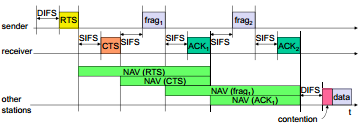
\includegraphics{fragmentation.png}

DFWMAC-PCF: 

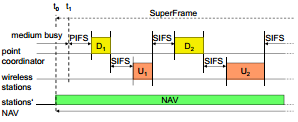
\includegraphics{dfwmac-pcf1.png}

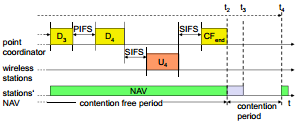
\includegraphics{dfwmac-pcf2.png}

\subsubsection{Management}

Association/Reassociation: integration into LAN, roaming -change networks by changing AP, scanning - active network search. Synchronization: timing. Power Management: periodic sleep without missing messages by frame buffering, traffic measurements. Management Information Base(MIB) - manage/read/write. Always associating with strongest signal could swamp AP or thrash between channels. Management packets aren't authenticated, can be spoofed.

Scanning: Passive - move to each channel and listen for beacons. Active:  Move to each channel and send Probe Requests to solicit Probe Responses from network.

Association: Request, Response, Data.

Roaming: Scan, Reassociaton request/response, AP signals new station to distribution system which updates location information and informs old AP to release resources.

Reassociation: Request, Verify Previous Association, Response, Send Buffered Frames, Data.

Infrastructure Synchronization:

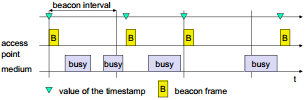
\includegraphics{infrastructuresynchronization.png}

Ad-Hoc Synchronization: 

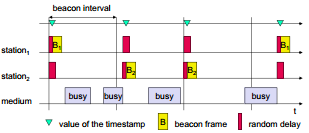
\includegraphics{adhocsynchronization.png}

Power Management: Switch not needed transceiver off. Timing Synchronization Function (TSF) – stations wake up at same time. Infrastructure - Traffic Indication Map(TIM) lists unicast receivers while Delivery Traffic Indication Map(DTIM) lists broadcast/multicast receivers. Ad-hoc - Ad-hoc Traffic Indication Map(ATIM) announces receivers by stations buffering frames so no AP(more complicated) and ATIM collisions possible.

\section{Network Layer and MobileIP}

Routing Protocols: Path selection for forwarding. Network Layer Protocol: Conventions for addressing conventions, packet format/handling. Control Protocols: error reporting, router signaling.

Functions: protocols in every host/router. Path Determination - algorithms route packets from source to dest.  Switching - move packets from router’s input to output. Call Setup - some network architectures require router call setup along path before data flows.

\subsection{IP Addresses}

IP Address: 32-bit identifier for host/router interface. Interface: connection between host/router and physical link, router have multiple interfaces, host has one. Subnet part high order bits, host part low order bits. Subnet - device interfaces with same subnet part of IP address and can physically reach each other without router. Classless InterDomain Routing(CIDR) - subnet portion of address arbitrary length with format a.b.c.d/x where x bits in subnet portion. Host get IP address hard-coded by system admin or Dynamic Host Configuration Protocol(DHCP) - dynamically get address from server. Network gets subnet from provider ISP address space. Hierarchical Addressing - route aggregation allows efficient routing information advertisement and more efficient routes. ISPs get address block from Internet Corporation for Assigned Names and Numbers(ICANN) - allocates addresses and manages DNS and assigns domain names and resolves disputes.

\subsection{Virtual Circuit vs. Datagrams}

Service Abstraction: guaranteed bandwidth, inter-packet timing preservation(jitter), loss-free/in-order delivery, congestion feedback to sender for channel. Most important network layer abstraction.

Virtual Circuits: Paths behaves like telephone circuit performance-wise and network actions. Call setup/teardown for calls before data flows, packets carries VC identifier(not destination host ID), every router path maintains state for passing connections, link/router resources(bandwidth/buffers) allocated to VC to get circuit-like perf. Initiate Call, Incoming Call, Accept Call, Call Connected, Data Flow Begins, Receive Data.

Datagram(Internet): No call setup at network layer. no network-level concept of connection(no state), packets routed using destination host ID, packets between same source-dest pair take different paths. Send Data, Receive Data.

Internet: Data exchanged among computers, elastic service with no strict timing req, smart end systems (computers) can perform cong. control and error recovery, simple inside network complexity at edge, many link types with different characteristics so uniform service difficult.

ATM: Evolved from telephony, human conversation has strict timing/reliability requirements need for guaranteed service, dumb end systems (telephones),complexity inside network.

\subsection{Routing Algorithms}

Determine good path from source to dest, graph nodes are routers, graph edges are physical links with cost(delay, dollar, congestion level). good path means minimum cost but other def’s possible. Max-flow algorithms used to find largest bandwidth path. Global: all routers have complete topology and link cost info(link state - LS). Decentralized: router knows link cost to physically connected neighbors , iterative computation process of, exchange of info with neighbors (distance vector - DS). Static: routes change slowly. Dynamic: routes change quickly with periodic update in response to link cost changes.

Link-State(Dijkstra's Algorithm): net topology and link costs communicated via link state broadcast, all nodes have same info, computes least cost paths(routing table) from one node to all other nodes, after $k$ iterations know least cost path to $k$ dest.s. $c(i,j)$ - link cost from node $i$ to $j$ and cost infinite if not neighbors, $D(v)$ - current path cost value from source to dest. $v$, $p(v)$ - predecessor node along path from source to $v$, $N$ - set of nodes with known least cost path. 

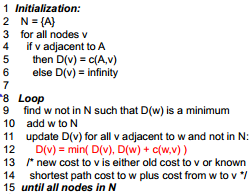
\includegraphics{dijkstra.png}

$n$ nodes $E$ links needs $O(nE)$ msgs each, $O(n^2)$ algorithm. Node can advertise incorrect link cost but each node computes own table. Troubleshoot by comparing local topologies. ISPS use this.

Distance Vector: Iterative - continues until no nodes exchange info and self-terminating, Asynchronous - nodes not exchange info/iterate in lock step. Distributed - nodes communicate with neighbors. Each node $x$ maintains cost $c(x,v)$ for each neighbor $v$, distance vector $D_x =[D_x(y): y\in{N}]$ containing $x$’s cost estimate to all destinations, distance vectors for each neighbor $v$ $D_v = [D_v(y): y\in{N}]$. Basic operation(Bellman-Ford) - $D_x(y) = min_v{(c(x,v)+D_v(y))}$ $y\in{N}$. 

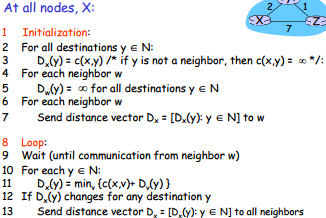
\includegraphics{distancevector.png}

Good news travels fast, bad news travels slow - count to infinity problem. Poisoned Reverse: If $Z$ routes through $Y$ to $X$ $Z$ tells $Y$ distance to $X$ infinite($Y$ won’t route to $X$ via $Z$). Convergence time varies, may be routing loops. Node can advertise incorrect path cost and each node’s table used by others so error propagate thru network. BGP uses this.

Hierarchical Routing: Can’t store 200 million dests in routing tables, exchange would swamp links. Internet is network of networks so each network admin controls routing in own network. Aggregate routers into autonomous systems(AS), routers in same(different) AS run same(different) intra-AS routing protocol. Gateway Routers: run intra-AS routing with other
routers in AS and inter-AS routing with other gateway routers.

\subsection{MobileIP}

Motivation: Routing -  physical subnet xhange implies IP address change for topological correct address or needs special entries in routing tables. Routing table change for forwarding  doesn't scale. Adjust host IP address is impossible to find mobile system, DNS updates take long time. TCP connections break. Security problems.

Requirements: Transparency - mobile end-systems keep IP address and communications continue after interruption with fixed network connection point changed. Compatibility - support same layer 2 protocols as IP so no current end-systems and router changes required and mobile end-systems communicate with fixed systems. Security - registration messages authenticated. Efficiency/scalability: little additional mobile system messages required with world-wide support of large number of mobile systems.

Terminology: Mobile Node(MN) - system that change connection point to network without changing IP address. Home Agent(HA) - router in MN home network that registers MN location and tunnels datagrams to COA. Foreign Agent(FA) - default router in MN foreign network of the MN that forwards tunneled datagrams to MN. Care-of Address(COA) - chosen address of current tunnel end-point for at FA/MN which is actual MN location from IP view point. Correspondent Node(CN)- communication partner.

Data Transfer: Sender sends to MN IP address, HA intercepts packet(proxy ARP) and tunnels to COA by encapsulation FA forwards the packet to MN. Receiver sends to sender IP address, FA default router. Not most efficient due to indirection but scales due to one contact point.

Integration: Agent Advertisement - HA/FA periodically send messages into physical subnets where MN listens and reads COA from FA advertisement. Registration(limited lifetime) - MN signals COA to HA via the FA and HA acknowledges MN via FA which are secured by authentication. Advertisement - HA advertises MN IP address (like fixed systems) and routers adjust entries which are stable for long time (HA responsible for a MN over long time) and packets to MN are sent to HA independent of COA/FA changes.

\subsection{Encapsulation}

Encapsulate one packet into another as payload like IPv6 in IPv4(6Bone), Multicast in Unicast(Mbone), IP-in-IP tunnel between HA/COA, minimal encapsulation, Generic Record Encapsulation(GRE). Optional Minimum encapsulation: avoids identical field repetition and only applicable for unfragmented packets.


\includegraphics{gre.png}

\subsection{Miscellaneous}

Optimization: Triangular Routing - sender sending packets via HA to MN has high latency and network load. Solutions - HA informs sender about HA location for direct tunneling but big security problems. FA Change - packets on-the-fly during change lost so new FA informs old FA to forward remaining packets and release resources.

Reverse Tunneling: MN sends to FA, FA tunnels packets to HA by encapsulation, HA forwards the packet to the receiver(standard case). Router accept only topological correct addresses(firewall, encapsulate by FA) and solves problems with multicast and TTL(TTL in home network correct but MN too far away from receiver) and enjoy home network services. Does not solve problems with firewalls since reverse tunnel can abused to circumvent security(tunnel hijacking) and optimization since packets tunneled via HA to sender(double triangular routing). Backwards compatible and extensions implemented easily and cooperate with current extensionless implementations ans agent advertisements carry reverse tunneling requests.

IPv6: security integrated and not add-on, registration authentication included, COA assigned via auto-configuration and every node has address autoconfiguration, no separate FA since all routers perform advertisement which can be used instead of special agent advertisement, co-located addresses, MN signals a COA sender directly so sending via HA not needed(automatic path optimization), soft hand-over without packet loss between two subnets, MN sends new COA to old router which encapsulates/forwards all packets for MN and forwards to new COA, authentication granted.

Problems: Security - authentication with FA since it belongs to another organization and no key management/distribution protocol  standardized in the Internet due to patent and export restrictions. Firewalls - cannot use with firewalls and special set-ups needed(reverse tunneling). QoS - tunneling makes it hard to give packet flows special treatment.

Security: Integrity - any changes to data between sender/receiver detected by receiver. Authentication - sender address really address of sender and all data received really data sent by sender. Confidentiality - only sender/receiver read data. Non-Repudiation - sender cannot deny sending data. Traffic Analysis - traffic and user profiles creation not possible. Replay Protection - receivers detect message replay.

Security Architecture: Multiple partners negotiate security mechanisms to setup security association, all partners choose the same parameters and mechanisms. Authentication-Header - guarantees packet integrity/authenticity and asymmetric encryption schemes guarantee non-repudiation. Encapsulation Security Payload(ESP) - protects confidentiality between communication partners. Mobile Security Association for registrations gives parameters for MN/HA/FA. Extended registration authentication. Replay registration prevention with  time stamps - 32 bit time stamps + 32 bit random number, and nonces - 32 bit random number(MH) + 32 bit random number(HA).

Key Distribution: FA has security association with HA, MN registers new binding at HA which answers with a new session key for FA/MN. 

Micro-Mobility Support: Efficient local handover inside foreign domain without involving HA which reduces control traffic on backbone, needed for route optimization. Cellular IP, HAWAII, Hierarchical Mobile IP (HMIP). Efficiency, Security, Scalability, Transparency, Manageability.

\section{Routing in Mobile Ad Hoc Network(MANET)}

Infrastructure-less, multi-hop, mobility changes routes, easy/fast deployment. Military environments with soldiers, tanks, planes. Personal area networking with cell phone, laptop, ear phone, wrist watch. Civilian environments with taxi cab network, meeting rooms, sports stadiums, boats, small aircraft. Emergency operations like search-and-rescue, policing and fire fighting. Assumption: fully symmetric environment where all nodes have identical capabilities and responsibilities. Route stability despite mobility, energy consumption. Some protocols invented for MANET, others adapted from previous wired protocols. No protocol good in all environments so some try adaptive protocols. Proactive Protocols - determine routes independent of traffic. Reactive Protocols - maintain routes when needed. Route Discovery Latency - proactive lower since routes maintained constantly while reactive higher since route from $X$ to $Y$ found only when $X$ sends to $Y$. Route Discovery/Maintenance Overhead - reactive lower overhead since routes determined only if needed while proactive higher(not necessarily) due to continuous route updating. Depends on the traffic/mobility patterns. Proactive(reactive) better static(dynamic) link overhead.

Flooding: Sender broadcasts packet $P$ to all neighbors, each node forwards $P$ to neighbors, sequence numbers avoid forwarding same packet more than once, $P$ reaches destination $D$ if reachable, $D$ does not forward  $P$. Pros - simplicity. Cons - high overhead. Many perform flooding of control packets used to discover routes instead of data packets. Control packet flooding overhead amortized over data packets between consecutive control packet floods.

Dynamic Source Routing(DSR): Node $S$ wants to send to node $D$ so initiates route discovery by flooding Route Request(RREQ), each node appends own identifier when forwarding RREQ, potential collision. $D$ sends a Route Reply(RREP) on route appended to RREQ reversed if links bi-directional. Unidirectional(asymmetric) links need route discovery for RREP piggybacking. IEEE 802.11 MAC need bi-directional links for ACKs. Default uses first route since easy to implement and indicates performance. Routes cached by any means which speeds up route discovery and reduces RREQ flooding. Source Routing - entire route included in packet header for forwarding. Route Error(RERR) sent when forwarding fails which updates route cache. Time/mobility invalidates caches which adversely affects performance(TCP) since several stale routes tried. Pros - reduces route maintenance overhead and caching reduces route discovery overhead while yielding many routes. Cons - packet header grows with route length due to source routing and RREQ floods reach all nodes and RREP from neighbors collide/storm and caches polluted with stale RREP, need invalid cache purge like static/adaptive timeouts based on link stability. Reduce RREPs by discriminating CW.

Ad Hoc On-Demand Distance Vector Routing(AODV): Maintaining routing tables at nodes to rid source routing. At most one next-hop per destination at a node(DSR have several routes for a destination). Nodes set up reverse path towards the source which assumes symmetric(bi-directional) links(asymmetric links due to different transmission power or interference). Intermediate nodes RREP for more recent path than one known to sender(destination sequence numbers), new RREQs assigned higher destination sequence numbers. Reverse(forward) path routing table entry purged after a timeout($active\_route\_timeout$) interval even if route still valid but unused. All active neighbors informed when next hop link breaks. RERR increments destination sequence number $N$, source initiates discovery with destination sequence number at least $N$, destination set sequence number to $N$ if lower. Reactive – failure to receive MAC-level ACK after several retries. Proactive – neighbors periodically exchange hello message whose indicated link failure. Sequence numbers prevent loop formation in RREQ when RERR lost. Expanding Ring Search - RREQs sent with small Time-to-Live(TTL) field to limit propagation then larger TTL when no RREP(DSR includes similar optimization).

Destination-Sequenced Distance Vector(DSDV): Nodes maintain routing tables with next hop, cost metric, destination sequence number used to avoid loop formation. Nodes periodically forward routing table to neighbors and increments/appends sequence number attached to route entries created for this node. $S(X)$/$S(Y)$ destination sequence number for node $Z$ as stored at node $X$ and sent by node $Y$ respectively. $S(X)>S(Y)$ $X$ ignores $Y$'s routing information. $S(X)=S(Y$) and cost of $Y$ smaller than $X$ $X$ sets $Y$ as next hop to $Z$. $S(X)<S(Y)$ $X$ sets $Y$ as next hop to $Z$ and $S(X)$ updated to equal $S(Y)$.

DSDV proactive so best no mobility. DSR(AODV) aggressive(selective) so best in low(high) mobility. DSR header bad or large networks. DSDV amortizes discovery cost so best for many destinations.

\section{Routing in Wireless Mesh Networks}

Improve network capacity for stationary nodes. Per-link delivery ratio product and bottleneck link throughput ignores hop count. End-to-end delay ghanges with network load as queue lengths vary causing oscillations.

Hop Count: Maximizes hop distance traveled which minimizes signal strength and maximizes loss ratio while higher Tx Power causes interference. Many shortest routes and intermediate loss rates.

ETX: predicted number of data transmissions to send packet over link, path ETX is sum of ETX link values over path. Expected probability of successfully received and acknowledged transmission is $d_fd_r$ where $d_f$($d_r$) forward(reverse) delivery ratio. ETX$=\frac{1}{d_fd_r}$. Delivery ratios affect throughput, detects asymmetry, uses(assumes) precise link loss measurements for finegrained decisions between routes, penalizes routes with more hops which have lower throughput due to inter-hop interference so assumes equal loss rates over links, minimize spectrum use which maximizes system capacity(reduce power) where nodes spends less time retransmitting. Values measured by broadcasting link probe packets with average period $\tau$(jittered by $±0.1\tau$), delivery ratio $r(t)=\frac{count(t-w,t)}{\frac{w}{\tau}}$ where $count(t-w,t)$ is probes received during window $w$ and $\frac{w}{\tau}$ is probe number expected. Each probe contains this information. More throughput advantage with smaller probe packets since larger packets have higher corruption chance, underestimates ACK delivery ratios and overestimates total transmission number per packet. Probes interfere with data so can significantly decrease throughput so piggyback on data for different probe sizes and accurate delivery rate. Pros - better than hop count, accounts for bi-directional loss rates, easily incorporated into routing protocols. Cons - only considers link loss rates and may not be best metric for mobility/power-limited/adaptive rate(multi-rate)/interference while predictions not always accurate and incur overhead and doesn't incorporate interaction between routing/ETX change causing oscillation and sub-optimal paths. 

Single radio nodes can not transmit/receive simultaneously, two radios tune to non-interfering channels, increased robustness due to diverse frequency fading characteristics, tradeoff between range and
data rate.

Weighted Cumulative Expected Transmission Time(WCETT): Multi-Radio Link-Quality source routing (MR-LQSR) - link-state  source routing protocol. Assume no power constraints, little mobility, nodes have multiple 802.11 radios tuned to noninterfering channels with fixed assignments.  Nodes discovers/measure neighbors links, floods information through network. Maximize throughput by prefering high-bandwidth/low-loss links, selecting short channel diverse paths. Expected Transmission Time(ETT) - ETT$=\frac{S}{B}$ETX with packet size $S$and link bandwidth $B$ so transmission lasts $\frac{S}{B}$ . Lower ETT implies better link. Use link sum as path metric(SETT) which favors short paths but ignores channel diversity. Interference reduces throughput which is lower if many links on same channel so path metric should be worse for non-diverse paths. Assumption all links on same channel interfere. Group links on path using channel, add link ETTs in each group, bottleneck group is with largest sum so too many links is poor quality(Bottleneck Group ETT - BG-ETT) which favors high-throughput/channel-diverse but ignores short paths, largest sum is path metric so lower value implies better path. WCETT $=(1-\beta)$SETT$+\beta$ BG-ETT, Higher(lower) $\beta$ more preference to channel diversity(shorter paths). Loss rate measured using broadcast probes link ETX updated every second, bandwidth estimated using periodic packet-pairs updated every 5 minutes. Provides performance gain even with one radio, channel diversity more important for shorter paths, throughput better for lower $\beta$, better than HOP/ETX, gains more prominent over shorter paths and light loads, optimal $\beta$ depends on load. Passive inference of loss rate and channel bandwidth, metrics measure link quality before changes which cause oscillation/sub-optimal performance and not globally good, need metrics for traffic impact on link quality and backoff overhead, WCETT assumes all links on path interfere(unrealistic), performance affected by more than routing metrics.

\section{Introduction to Sensor Networks}

Large number of low-cost/power, multifunctional, small sensor nodes consisting of sensing, data processing, communicating components. Node positions need not be pre-determined, protocols/algorithms self-organizing. Failure prone, frequent topology changes, broadcast communication whereas(most ad hoc networks use point-to-point), limited computation/memory, no global ID. collect/route data to sink which communicates with task manager via Internet/Satellite. Design factors: fault tolerance, scalability, production costs, operating environment, network topology, hardware constraints, transmission media, power consumption.

Hardware Constraints: Sensing Unit - composed of two subunits(sensors and analog to digital converters - ADCs). Processing Unit - manages collaboration procedures to carry out tasks. Transceiver Unit - connects to network. Power Units  - most important. Location Finding System - routing techniques and sensing tasks require high accuracy location knowledge. Mobilizer - move sensors. Matchbox-sized module, consume extremely low power, operate in high volumetric densities, have low production cost, dispensable, autonomous, adaptive. Sink/sensor protocol stack has Power/Mobility/Task Management Plane spanning application, transport, network, data link, physical.

Topology: Pre-Deployment and Deployment Phase – thrown in mass or placed one by one in sensor field. Post-Deployment Phase - topologies prone to frequent changes. Re-Deployment Phase – addition new nodes poses and reorganize network.

Environment: Micro-sensors, onboard processing, wireless interfaces feasible at very small scale can monitor phenomena up close which enables spatially/temporally dense environmental monitoring. Embedded Networked Sensing reveal previously unobservable phenomena.

Transmission Media: Industrial Scientific and Medical(ISM) Bands – 915 MHz ISM band widely suggested and most countries offer license-free communication. Infrared – license-free and interference robust but requires line of sight between sender/receiver. Ultra Wide Ban(UWB).

Power Consumption: Limited power source (<0.5 Ah 1.2V), lifetime strong dependent on battery lifetime, power consumption divided into three domains(sensing, communication, and data processing).

Large scale sensor networks require richer inter-node communication for In-network storage/processing/routing. Need point-to-point routing to scale to flows and different densities. Design goals are simple(minimum state), scalable(low control overhead, small routing tables), efficient(low routing stretch), and robust against node failure.

Greedy Perimeter Stateless Routing(GPSR): DSR/AODV suffer from out of date state and Hard to scale, use geographic information for routing by assuming every node knows position(x,y) and keep less network state in the network and requiring fewer update messages. Select neighbor geographically closest destination as next hop so keep state for neighbors. Beaconing mechanism provides all nodes with neighbors’ MAC/positions and minimize costs by piggybacking. Right Hand Rule - next edge traversed is sequentially counterclockwise about node $x$ from edge $(x,y)$ when arriving at $x$ from node $y$(traverse exterior region in counter-clockwise edge order). Planar Graph - graph in which no two edges cross. Relative Neighborhood Graph(RNG) - $\forall{w\neq{u,v}}: d(u,v)\leq{max[d(u,w),d(v,w)]}$. Gabriel Graph(GG) - $\forall{\neq{u,v}}:d^2(u,v)<[d^2(u,w) + d^2(v,w)]$. Use greedy forwarding whenever possible, resort to perimeter routing when greedy forwarding fails, resume greedy forwarding when we are closer to destination. Implementation support MAC-layer feedback ,interface queue traversal, promiscuous network interface use, graph planarization. Pros - Low routing state and control traffic so scalable and handles mobility. Cons - GPS location not available everywhere and geographic distance doesn't correlate with network proximity and overhead in location registration/lookup and planarization algorithm limitations(works under unit disk model which doesn’t hold in practical network and hard to handle mobility snd reduces network connectivity) and localization expensive and nodes need to update location somewhere.

Beacon Vector Routing(BVR): Create routing gradient from connectivity information rather than geography, assign positions based on connectivity and greedily forwarding on this space. Deriving Positions - $r$ beacon nodes $(B_0,B_1\dots{,B_r})$ flood network so node $q$’s position $P(q)$ is hops to each beacon $P(q) = (B_1(q), B_2(q),\dots{,B_r(q)})$ and $q$ advertises coordinates using $k$ closest beacons $C(k,q)$ so nodes know neighbors’/beacon positions. Forwarding - $dist_k(p,q)=\sum_{i\in{C(k,q)}}\omega_i{|B_i(p)-B_i(q)|}$ choose neighbor to reduce $dist_k(*,q)$ to reach $q$ but enter Fallback Mode(route towards beacon closer to destination) when no neighbor improves and scoped flood when Fallback fails and beacon reached. Each entry beacon vector has sequence number periodically updated by beacon between timeout so non-beacons nominate themselves as beacons when beacons $<r$. Store location mapping at beacons with hashing (H: nodeid $\rightarrow$ beaconid) so node $k$ wanting to be destination periodically publishes coordinates to beacon $b_k=H(k)$ and route to $k$ with lookup request to $b_k$ with coordinates cached. Can achieve performance comparable to true positions, beaconing overhead grows slowly with network size (less than 2\% nodes for larger networks), great benefit for deriving coordinates from connectivity, average stretch consistently low($<1.1$), robust to obstacles unlike geographic forwarding, costly floods but low density resilient, coordinates stable with few/small, sustained high throughput. Simple/robust/scalable/efficient so using connectivity for deriving routes is good for low density/obstacles, implementation indicates can work in real settings. Routing/transmission stretches high and no delivery guarantee with scoped flooding since may collide from multiple sources.

\section{Delay Tolerant Networks(DTN)}

Rural area(buses, mail trucks, infostations), Mobile routers with disconnection, Sensor networks, Deep space, Underwater, etc... Internet exists some end-to-end path with RTT At most a few seconds(typically less than 500 ms) and use retransmission for reliability and packet switching right abstraction. DTN May not exist e2e path with contact connectivity intermittent and arbitrary with large delay (hours, days) and high hink error and low capacity with resource budget limiting transmissions and different network architectures. Issues in naming, addressing, location management, dynamic graph routing, scheduling, security, applications, etc... Routing on time-varying topology have links unpredictable so use any/all links. Inputs topologies, traffic demands, vertex buffer limits, mobility patterns to determine route/schedule to optimize some metric(delay, throughput, resource consumption).

Flooding: Node forwards any non duplicated msg to any other node encountered. Pros - low delay. Cons - high transmission overhead and replicates messages after copy delivered.

Direct Contact: Source holds data until contact with destination. Pros - minimal resources. Cons - long delay.

Simple Replication: Source sends $r$ identical copies over first $r$ contacts which Relay directly to destination so low average-case delay.

History-Based Replication: Nodes track message delivery probability for another node and replicates to $r$ highest ranked relays. Record contact duration and inter-contact time for contact probability. Replicates messages after copy delivered. Simple relays relay once while history relays relay multiple times.

Erasure-Coding Based Replication: Split/distribute messages to more contacts to increase delivery chance instead of seeking good contacts. Same bytes number flow in network now in coded blocks which makes order insignificant. Given replication factor $r$ any $\frac{1}{r}$ blocks reconstruct original data. Leveraging more contacts reduces worse-case latency – risk of outlier bad contacts. Use first $rk$ relays each get $\frac{1}{k}$ copy so $\frac{k}{rk}$ relays to succeed. $k\geq{1}$ reatled to coding algorithm. Delay distribution converges to constant when $k$ large so almost assured constant delay. Low success rate with small deadlines, high success rate for longer deadlines(due to lower 99th percentile latency distr), few very low delay cases.

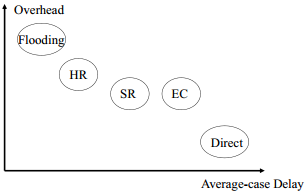
\includegraphics{dtnsummary1.png}

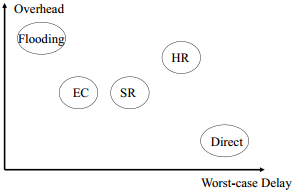
\includegraphics{dtnsummary2.png}

Enhancements: Optimize common case and guarantee worst-case. Replicate currently based on first $r$ contacts but Could use delivery probability for selection, replicate quantity currently every node selected replicated equal amount but could use delivery probability for deciding amount, adapt coding parameters based on delivery probability and performance requirement, apply network coding, adapt/quantity/when to replicate based on message urgency.

\section{Transport Layer}

Provides logical communication between app processes on different hosts, runs in end systems. Send Side - breaks app messages into segments and passes to network layer. Rcv Side - reassembles segments into messages and passes to app layer. Internet uses TCP/UDP. Network Layer - logical communication between hosts. Transport Layer - relies/enhances network layer services. UDP - unreliable/unordered so no-frills extension of best-effort IP. TCP - reliable/in-order delivery with congestion/flow control and connection setup. Delay/bandwidth guarantees unavailable. Demultiplexing at Rcv - deliver received segments to correct socket. Multiplexing at Send -gather/envelope data from multiple sockets with header. Host receives IP datagrams with source/destination IP address, 1 transport-layer segment, source/destination port number. Host uses IP addresses and port numbers to direct segment to socket. Connectionless - create sockets with port numbers identified by (dest IP address, dest port number) and checks destination port number then directs UDP segment to socket with port number when host receives segment thus IP datagrams with different source IP addresses and port numbers directed to same socket. Connection-Oriented - TCP socket identified (source IP address, source port number, dest IP address, dest port number) used by receiver to direct segment to socket so server supports many simultaneous sockets and have different sockets for each client(non-persistent HTTP have different sockets for each request). Client Client- Create socket with socket() system an connects socket to server address using connect() and send/receive data using read()/write(). Server Side - create socket with the socket() and bind socket to address using bind()(Internet server socket address consists of port number on host machine) and listen for connections with listen() and accept connection with accept()(blocks until client connects with server and send/receive data.

UDP: no frills bare bones Internet transport protocol with best effort service so segments may lost/reordered to app. Connectionless - no handshaking between sender/receiver and segments handled independently. No connection establishment decreases delay, simple with no connection state at sender/receiver, small segment header, no congestion control so blast away as fast as desired. Used for streaming multimedia apps(loss tolerant rate sensitive), DNS, SNMP. Add reliability at application layer. 

Checksum: Detect errors(flipped bits) in segment. Sender -treat segment as 16-bit integers sequence for 1’s complement sum and puts checksum value into checksum field. Receiver - compute checksum and check if equals checksum field value (NO - error detected, YES - no error detected). Carryout from most significant bit added to result(ignores endianness). Easy computation with incremental update and endian-independent. 
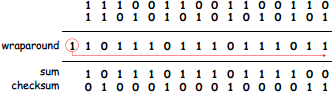
\includegraphics{checksum.png}

Unreliable channel characteristics determines reliable data transfer protocol complexity, checksum + NACK/ACK over eror channel, sequence no. + timeout over lossy channel. Stop-and-Wait works with stinky performance utilization $U_{sunder} = \frac{\frac{L}{R}}{RTT + \frac{L}{R}}$, $L$ bits packet length, $R$ bps transmission rate, network protocol limits physical resource use. Pipelining - sender allows multiple unacknowledged pkts in flight so increase sequence number range with buffering sender/receiver.

Go-Back-N: $k$-bit seq number in pkt header, window up to $N$ consecutive unack’ed pkts allowed. ACK(n) - ACKs all pkts up to including seq number $n$(cumulative ACK) and may receive duplicate ACKs. Time each in-flight pkt with timeout(n) - retransmit pkt n and all higher seq number pkts in window.

Selective Repeat: Receiver individually acknowledges correctly received pkts and buffers pkts in-order delivery to upper layer. Sender resends pkts for which ACK not received(timer for each unACKed pkt) with $N$ consecutive seq numbers window and limits unAcked pkts' seq numbers. Sender - send pkt when data from above and next available seq number in window and resent packet $n$ and restart timer when timeout(n) and mark pkt $n$ received and advance window base to next unACKed seq number if $n$ smallest unACKed packet when ACk(n) in $[sendbase, sendbase+N]$. Receiver - send ACK(n) when $[rcvbase-N,rcvbase-1]$ and buffer out-of-order or deliver in-order (also deliver buffered) then advance window to next not-yet-received pkt when pckt $n$ in $[rcvbase, rcvbase+N-1]$  and ignore otherwise.

Reliable Data Transfer Mechanisms: Checksum - detect bit errors. Timer - detect packet loss at sender. Sequence Number - Detect packet loss/duplicates at receiver. ACK(NACK) - inform sender pkt (incorrectly) received. Window/Pipelining - increase throughput and adapt to receiver buffer size and network congestion. NACK speeds up timeouts.

Congestion Control: Too many sources sending too much data too fast for network to handle. Manifestations through lost packets(buffer overflow at routers) and long delays(queuing in router buffers). One router with infinite buffers and no retransmission see large delays at maximum achievable throughput. one router with finite buffers and lost packet retransmission see more work(retrans) for given goodput and unneeded retransmissions since link carries multiple pkt copies. $\lambda_{in}$ original data, $\lambda'_{in}$ plus retransmissions, goodput($\lambda_{in}=\lambda_{out}$), perfect transmission only when loss($\lambda'_{in}>\lambda_{out}$), retransmission of delayed packet makes $\lambda'_{in}$ larger (than perfect case) for same $\lambda_{out}$. Multihop paths with timeout/retransmit see upstream transmission capacity wasted when packet dropped. End-End - no explicit network feedback so congestion inferred from end-system observed loss/delay (approach taken by TCP). Network-Assisted - routers provide feedback to end systems with single bit indicating congestion (SNA, DECbit, TCP/IP ECN, ATM) or explicit sned rate(XCP).

TCP: Point-to-point with one sender/receiver, reliable/in-order byte steam with no message boundaries, pipelined with congestion/flow control that set window sizes, send/receive buffers, full duplex data so bi-directional data flow in same connection(maximum segment size MSS), connection-oriented with handshaking (exchange control msgs) init’s sender/receiver state(sequence numbers, buffers, RcvWindow) before data exchange, flow controlled so sender not overwhelm receiver. Three Way Handshake - client host TCP SYN segment to server which specifies initial seq number with no data then server receives SYN and replies with SYNACK segment allocating buffers and specifies initial seq. number then client receives SYNACK and replies with ACK segment which may contain data(SYNCookie allows server allocate state after client's ACK). Closing Connection - client sends TCP FIN segment to server then server receives FIN and replies with ACK and closes connection and sends FIN then client receives FIN and replies with ACK and enters timed wait to respond with ACK to FINs then server receives ACK connection closed. Handles simultaneous FINs with modification. Seq. numbers are byte stream numbers of segment data's first byte. ACKs are seq number of next byte expected(cumulative). TCP spec doesn’t say how to handle out-of-order segments so up to implementer. Timeout value longer than varying RTT, too short - premature timeout and unnecessary retransmissions, too long - slow reaction to segment loss. SampleRTT -measured time from segment transmission until ACK receipt (ignore retransmissions since ACKs ambiguous). EstimatedRTT $= (1-\alpha)$EstimatedRTT$+ \alpha$SampleRTT, exponential weighted moving average so influence of past sample decreases exponentially fast($\alpha{=0.125}$).  EstimatedRTT large variation needs larger safety margin, estimate of how much SampleRTT deviates from EstimatedRTT($\beta{=0.25}$) with DevRTT$=(1-\beta)$DevRTT$+\beta{|}$SampleRTT$-$EstimatedRTT$|$ then set TimeoutInterval$=$EstimatedRTT$+4$DevRTT. Sender - create segment with seq number of first data byte in segment then start timer if not already running(timer for oldest unacked segment) when data from app and retransmit segment then restart timer when timeout and if acknowledges previously unacked segments then update known acks and start timer for outstanding segments when ack. Receiver - wait up to 500ms for next segment but if no next segment then send ACK when in-order segment arrive with expected seq number and all data up to number ACKed or immediately send single cumulative ACK fro both in-order segments when in-order segment arrive with expected seq number and another segment has ACK pending or immediately send duplicate ACK next expected byte when out-of-order segment arrive with higher-than-expect seq. number(gap detected) or immediately send ACK if segment starts at gap's lower end when segment arrive that fills gap. Time-out period incurs long delay before resending lost packet so detect lost segments via duplicate ACKs since sender sends segments back-to-back have many duplicate ACKs for lost segment. Assumes segment after ACKed data lost on 3 ACKS for same data, Fast Retransmit  - resend segment before timer expires. Flow Control - sender won’t overflow receiver’s buffer by transmitting too much too fast with speed-matching service by matching sending rate drain rate and rcvr includes RcvWindow value in segments so sender limits unACKed data to RcvWindow and guarantees receive buffer doesn’t overflow. Congestion Control - sender transmit as fast as possible without congesting network and decentralized so senders probe bandwidth by implicit feedback of ACK(segment received, network not congested, increase sending rate) or lost segment (assume loss due to congestion, decrease sending rate) since available bandwidth changes depending on other connections and limits rate by unACKed bytes in pipeline (LastByteSent-LastByteAcked $\leq$ cwnd, cwnd dynamic function of perceived network congestion) and min(cwnd,rwnd) with $rate=\frac{cwnd}{RTT}$ roughly so  timeouts cut cwnd to 1 and 3 duplicate ACKs cut cwnd in half(less aggressively since some segments getting through) also Slow Start increases cwnd exponentially fast at connection start or following timeout at 1 MSS then quickly ramp up to respectable rate by doubling cwnd every RTT through incrementing cwnd by 1 for every ACK and Congestion Avoidance increase cwnd linearly when cwnd $>$ ssthresh by increase cwnd by 1 MSS per RTT to approach congestion slower than slow start implemented by $cwnd=cwnd+\frac{MSS}{cwnd}$ for each ACK received(Additive Increase Multiplicative Decrease - AIMD)so in summary sender in slow-start(congestion-avoidance) phase with window grows exponentially(linearly) when CongWin $<$($>$) Threshold and Threshold $:=$ CongWin/2 and CongWin $:=$ Threshold(1 MSS) when triple duplicate ACK(timeout) occurs.

\section{TCP in Wireless Networks}

\subsection{Transmission Errors}

Random Errors: Cause fast retransmit unnecessary reduces congestion window and throughput. Cause timeout when multiple packet lost with TCP-Reno and Selective ACK(SACK) to lesser extent.

Burst Errors: Window worth of data lost when wireless link unavailable for extended duration from passing truck or driving through tunnel. Timeout results in long idle time and slows start, which unnecessarily reduces congestion window to 1 MSS and ssthresh to 1/2.

Hide Loss: Link level Mechanisms, Split Connection Approach, TCP-Aware Link Layer, TCP-Unaware Approximation of TCP-Aware Link Layer. Find Loss Reasons: Explicit Notification, Receiver/Sender-Based Discrimination.

Link Layer Schemes: Recover wireless losses using FEC code, retransmission, and adapting frame size. Hide wireless losses from TCP sender so Link layer modifications needed at both ends of wireless link so TCP need not modified. Reliable link layer beneficial to TCP if provides in-order delivery and TCP retransmission timeout large enough to tolerate additional link level retransmits delays. Most widely used since easy and most links already do.

Split Connection Approach: End-to-end TCP connection broken into one connection on wired part and one over wireless part. Hides transmission errors from sender with responsibility at base station and if specialized transport protocol on wireless needs wireless host modification.  Advantages - local/fast error recovery due to shorter RTT on wireless link and  BS-MH connection optimized independent of FH-BS connection with different flow/error control two connections and good performance using appropriate BS-MH protocol since standard TCP on BS-MH performs poorly when multiple packet losses occur per window (timeouts occur on BS-MH connection, stalling during the timeout) but improve through selective acks. Disadvantages - end-to-end semantics violated since ack delivered to sender before data delivered to receiver and not useful if data/acks traverse different paths (both don't go through BS) and Extra copy/storage required at BS so not widely used.

TCP-Aware Link Layer: Snoop Protocol retains local recovery and end-to-end semantics, BS soft state instead of hard state. BS buffers packets to allow link layer retransmission and retransmit on wireless link when dupacks received from MH and prevent fast retransmit at TCP sender by dropping dupacks. If wireless link level delay-bandwidth product $<4$ packets then simple(TCP-unaware) link level retransmission scheme suffices since can deliver lost packet without 3 dupacks from TCP receiver since delay-bandwidth product small. Hides wireless losses from the sender and requires BS modification(network-centric approach). Advantages - high throughput achieved and improved using selective acks with local recovery from wireless losses and fast retransmit not triggered at sender despite out-of-order link layer delivery and End-to-end semantics retained with soft state at base station so state loss affects performance not correctness. Disadvantages - link layer at base station needs TCP-aware and not useful if TCP headers encrypted (IPsec) and can't use if TCP data/acks traverse different paths (both don't go through BS).

TCP-Unaware Approximation of TCP-Aware Link Layer: Delayed Dupacks Protocol imitates Snoop without BS TCP-aware. TCP receiver delays dupacks (third and subsequent) when out-of-order packets received intended to give link level retransmit time. Pros - recovery from  transmission loss without triggering TCP sender sender. Cons - Recovery from congestion losses delayed.

Explicit Notification: BS tags dup-ack with Explicit Congestion(Loss) Notification ELN(ECN) if wireless(congestion) related loss.  Preferred over receiver/sender discrimination. 

Receiver-Based Discrimination - Receiver guess packet loss cause. Sends notification to TCP sende when receiver believes packet loss due to errors. On notification TCP sender retransmits the packet without reducing congestion window.

Sender-Based Discrimination: Sender determine packet loss cause. Don't reduce congestion window if packet loss due to errors.

\subsection{Mobility}

Hide mobility from TCP sender or Make TCP adaptive to mobility. 0(1)-second Rendezvous Delay - beacon arrives 0(1) second after cell boundary crossed. TCP performance degradation in overlapping cells due to encapsulation/forwarding delay during handoff, additional degradation in non-overlapping cells due to packet sender loss and idle time. When MH the TCP receiver then after handoff complete sends 3 dupacks to sender which this triggers fast retransmit(special notification could replace dupacks), when MH is TCP sender fast retransmit after handoff completion. Smooth Handoffs - avoid packet loss with sufficient overlap between cells or buffer packets at BS and forward the packets to new BS before packets discarded after short interval.

M-TCP: Avoid shrinkage in the congestion window due to fast retransmit. Sender enters persist mode when new ack received with receiver’s advertised window 0 and doesn't send data before persist timer expires. exits persist mode when positive window advertisement received. RTO/cwnd same as before. Splits TCP connection into two logical parts with independent flow control as I-TCP. BS doesn't send to FH unless BS received ack from MH wich maintains end-to-end semantics. BS withholds ack for last byte acked by MH which sent with window advertisement 0 if MH moves away (handoff in progress) to put sender FH into persist mode. Last ack not withheld if BS doesn't expect other acks from MH when BS has no other unacked data buffered locally, prevents sender timeout at end of transfer(burst of data). Route changes with mobility and new route more congested so starting full speed after handoff not obvious right.

Mobile Ad Hoc Networks: Improve throughput by informing TCP of route failure by explicit message and let TCP know when route repaired with probing or explicit notification. Reduces repeated TCP timeouts/backoff. Route discovery returns cached route and TCP sender transmits after timeout but cached route broken, process repeats until good route found. Caching speeds route repair but incorrect repairs degrades caching performance so need mechanisms for determining when cached routes stale. Caching reduce route discovery overhead but low cache accuracy cause routing overhead gains offset by TCP performance loss due to multiple time-outs.     

\section{Localization: Algorithms and System}

\textbf{Applications}: Location aware information services like E911, location-based search, target advertisement, tour guide, inventory management, traffic monitoring, disaster recovery, intrusion detection. Scientific applications like air/water quality monitoring, environmental studies, biodiversity. Military applications. Resource selection like server, printer. Sensor networks for geographic routing since sensing data meaningless without knowing location. Location availability enables new applications. \textbf{Signals for localization:} RF signal: WiFi, Bluetooth, sensor, UWB. Acoustic signal(TOF), Ultrasound, Light(intensity), Magnetic Field(intensity through gyroscopes), IMU. \textbf{Ongoing work on localization}: Device free localization, localization in mobile networks, combine other signals to improve localization accuracy, gesture/activity recognition. \textbf{Beyond Localization}: Xbox Kinect, WiFi based tracking, light based tracking, Google tracking, audio based tracking.

\subsection{Single Hop Wireless Networks}

\subsubsection{Global Positioning System(GPS)}

\textbf{History}: US Defense Department wants very precise navigation. 1973 US Air Force proposed Navigation System with Timing and Ranging: Global Positioning System (NAVSTAR GPS) using satellites. \textbf{Goals}: time, position, velocity, local time, distance, arrival time. \textbf{Overview}: GPS satellites are set of wireless base stations in sky that simultaneously broadcast beacon messages.  GPS receiver measures arrival time to satellites, and triangulates its position. \textbf{Need 4 satellites since receiver clock isn't synced with satellites}, $t^{R1}=t^S+\frac{|p-p_1|}{c}+\delta_{clock-drift}\implies{|p-p_1|=c(t^{R1}-t^S-\delta_{clock-drift})}$. Pseudo range $c(t^{R1}-t^S)$. Each satellite timestamps transmission and receivers measure received time for transmission time, correct satellite location, radio wave speed, arrival time. \textbf{Requirements}: all 24 satellites transmit on same two frequencies but use different codes, jamming resistant, spoofing resistant, allows military access control of access (selected availability), satellites provide their positions. \textbf{DSSS/CDMA modulation.} \textbf{Navigation message}(37,500 bits) transmitted on L1/L2 at 50bps consisting of satellite status and clock information. \textbf{Two types of clock signals}: Coarse/Acquisition(C/A) Code available for civilians on L1 that provides 300m resolution and Precise(P) Code on L1/L2 for military that provides 3m resolution. Encrypted P Code provides selected availability and anti-spoofing. Receiver use C/A code on L1, timing information and computes pseudo-ranges. \textbf{Denial of Accuracy(DOA)}: US military prohibit full system resolution by Anti-Spoofing(AS) - P code encrypted - and Selective availability(SA) - noise added to clock signal. Segments(components): space - satellite constellation, control - satellite control, user - users with receivers. \textbf{Space Segment:} 24 satellites in operational mode, 21 in use, 3 for testing, Altitude - 20200Km with 12hr periods, Current Satellites - Block IIR 25,000,000 at 2000 KG with hydrogen maser atomic clocks that lose one second every 2,739,000 million years. \textbf{Control Segment:} Master Control Station located at Consolidated Space Operations Center(\textbf{CSOC}) Flacon Air Force Station Colorado Springs, track satellites for orbit and clock determination, yime synchronization, navigation message upload, and DOA management. Simplest topology for localization system. \textbf{Limitations}: Hardware requirements vs. small devices, obstructions common since each node needs LOS to 4 satellites which is hard to achieve(urban canyon, indoors, and underground), jammed/spoofed, power-hungry. Low-orbiting satellites allow GPS indoors but isn't widely used.

\subsubsection{War-Driving}

GPS not prevalent as WiFi. \textbf{Goals}: High coverage and accuracy (<10m) outdoor/indoor. No new infrastructure, low cost, APs broadcast beacons, war drivers already build AP maps calibrated using GPS and constantly updated. Indoor WiFi positioning gives 2-4m accuracy but requires high calibration overhead(10+ hours per building). \textbf{War-driving:} driving around looking for wireless networks. Metropolitan-scale location with reasonable accuracy using 802.11 based positioning. Evaluate several location algorithms as war driving data ages, as calibration data noisy, As calibration data amount reduced. \textbf{Training phase: }Collect AP beacons by war driving with Wi-Fi card and GPS where each scan records GPS coordinate and AP list, covers one neighborhood in 1hr to build radio map from AP traces. \textbf{Positioning phase:} position user with radio map amd compare with GPS. \textbf{Algorithms}: \textbf{Centroid} – positions weighted average of all heard APs, \textbf{Fingerprinting} - user hears APs with signal strength signature so find top $k=4$ fingerprints with closest match in APs seen and corresponding RSS (\textbf{RADAR} compares using absolute signal strengths, \textbf{RANK} compares using relative signal strength identity ranking of signal strengths) to determine user location as average of $k$ fingerprints locations, \textbf{Particle Filters} - probabilistic approximation algorithm for Bayes filter. AP density matters so algorithms effects larger in sparse topologies. Rank performs worst. More APs/scan means lower median error and Rank does not work with 1 AP/scan. Minimal effect on accuracy even with $50\%$ AP turnover. Particle filter and centroid less sensitive to GPS noise.\textbf{Wifi Localization summary:} WiFi-based location has low calibration overhead. Positioning accuracy depends on AP density so dense means better accuracy. Urban area, simple algorithm(centroid) yields same accuracy as complex ones. AP turnovers and low training data density do not degrade accuracy. GPS noise only affects fingerprint algorithms.

\subsection{Multihop Wireless Networks}

\subsubsection{Sextant}

Given $n$ points with $k$ positions and $m$ distances between pairs known, find point positions. Find locations to satisfy under-constrained distance constraints: Modify graph to avoid being under-constrained, find most likely positions, or find all possible positions. Localization accuracy depends constraint extraction, solve constraints set to produce estimated location set $\epsilon_A$. \textbf{Absolute constraints} on landmark nodes are explicit coordinates or regions. \textbf{Relative constraints} are connectivity information between nodes, use two radii to handle irregular wireless transmission zones and incorporate rss and angle info. Boolean packet received/not-received, reachable/unreachable nodes $\leq{R}$/$\geq{r}$ away. \textbf{Positive constraints:} $A$ must be inside region $X$, intersection $\epsilon_A = \epsilon_A\cap{X}$. \textbf{Negative constraints}: $A$ cannot be inside region $X$, subtraction $\epsilon_A = \epsilon_A-X$. Maximal wireless coverage region union all circles of radius $R$, Assured wireless coverage region intersection all circles of radius $r$. $\Gamma_x$ set of positive constraints learned from neighbors. $\Theta_x$ set of negative constraints learned from non-neighbors, Invariant: location estimate $\mathcal{E}_x= \bigcap_{\rho\in\Gamma_x}\rho-\bigcup_{n\in\Theta_x}n$. Measurement inaccuracies could result in $\emptyset$ after constraints intersect. More anchors may over-constrain system so may need to find closest solution. \textbf{Represent regions} with polygons enclosed by knotted Bezier curves defined by 4 control points that expressive and compact, able to handle non-convex and holey shapes, and enables efficient region operations(union, intersect, subtraction). \textbf{Protocal:}\textbf{Neighborhood discovery} by nodes transmit periodic beacons with threshold reception required for boolean connectivity. Each node $B$ keeps track of estimated location set $\epsilon_B$ and positive constraints/negative constraint sets.  Positive information used at first hop, negative information used within first few hops. \textbf{Evaluation} Compare against triangulation by neighbor nodes centroid, single-hop with no transitive dissemination, positive constraints with no negative information. Error metrics with Monte Carlo technique by randomly choose sample points in region and pick point that minimizes average distances to other sample points. Sextant locates more nodes and requires fewer landmarks for given accuracy requirement. Sextant performance effective over wide sensing range values.\textbf{conclusions:} High accuracy and scalability with conservative/comprehensive extraction of negative/positive constraints and transitive constraint dissemination and explicit region representation using Bezier curves and use events to refine node location. Unifies node/event localization in same framework. Evaluation via simulation and experiments that deals with simplistic assumptions violations. Implemented on MICA-2 motes, PDAs and laptops.\textbf{Pros} 1. Extract negative constraints. 2. Use region to represent location. 3. Use efficient replication of regions. \textbf{Improve:} Solve the problem of empty intersection.

\section{RFID}

\textbf{UPC}: 1932 Wallace Flint first suggested automated checkou, UPC bar code formats developed in next 30 years, April 3 1973 grocery industry adopted UPC, computerized scanning/inventory, UPCs ubiquitous. UPC insufficient to many applications like cattle stock monitoring, person identification, tracking children and patients, highway toll collection, remote keyless entry, vehicle parking monitoring, toxic waste monitoring, asset management, local positioning systems.

\textbf{RFID} tags transmit signals and receivers estimate tag location
by measuring signal‘s time of flight. Radio Frequency Identification not a specific technology but an entire class of tagging items by radio accomplished through a variety of means. RFID been much hyped recently as replacement for UPC and more but privacy/security concerns have cropped. WWII roots when British put IFF(Identification: Friend or Foe) transponders in planes for returning aircraft identification. 1970s Los Alamos RFID tagged nuclear equipment and personnel for safety. Amtech/Identronix spun off released research. Cattle stock monitoring/tracking through railroads, fleet vehicle identification (tractors/trailers/cargo), highway toll collection on highways, remote keyless entry. 1984 several manufacturers/flavors.\textbf{RFID System} RFID tag/transponder has Antenna, wireless tranducer, encapsulating material. Passive tags has power induced by magnetic field of RFID reader feasible up to 3m and low price. Active tags have on-chip battery for 100m. RFID reader/transceiver has antenna, transceiver, decoder. Data processing subsystem. Security application dependent with no crypography. Available on many products/vendors. Connection set-up time depends on product and medium access scheme typically 2ms per device. No QoS. Manageability very simple like serial interface. \textbf{Advantage}: extremely low cost, high volume available, no power for passive RFIDs, large  products variety, 300 Km/h relative speeds, broad temperature range. Disadvantage: no QoS, simple DOS, crowded ISM bands, typially one-way ID activation/transmission. Function: Standard - tags respond to radio interrogation signal from reader by transmitting ID, Enhanced - data sent to the tags with different media access schemes.  Features: No LOS and tags withstand difficult environmental conditions and available with read/write memory with smart-card capabilities. Programmability: WORM(write once read many times) at manufacture/installation, Direct Contact/RF(reprogrammable 10,000-15,000 times), Full Read/Write. \textbf{Performance Metrics}: access rate - number tags reliably read per unit time, accuracy- percentage tags read reliably in given duration, energy usage - tags/sensors/readers. Tradeoff between accuracy and access rate. \textbf{ Multiple tags} on object enhances reliability where reader can treat simultaneous transmissions from multiple tags as single transmission in multipath environment. Write by explicit association where different RFIDs on object contain different IDs and use external database to map IDs to object or implicit association where a few bits in ID reserved to distinguish tags on object or use timestamp to implicitly differentiate between tags. Multiple tags improve localization by extracting constraints for each individual tag and that bound distance between tags. Readers getting cheaper and multiple readers required to cover area nad support concurrent reads. Collisions from multiple reader interference so assign different channels, use direction antennas, control transmission power, develop MAC protocol to minimize collisions. \textbf{Non-cooperative tag} access with implicit communication by writing to and reading from tags.\textbf{ Cooperative tag} access when readers communicate with each other to decide which readers read which tags. \textbf{RFID network generates lots of data} so aggregate before transmission like reporting max, min, mean, median by removing redundant data collected by nearby readers. Different from sensor network aggregation  since sll sensors low-end vs. powerful reader and low-end tags decide intelligence in tags/readers. Security by obscurity does not work so use standard cryptographic algorithms with sufficient key lengths. \textbf{RFID-enabled passport:} Metallic anti-skimming material added in cover/spine to reduce read distance to 1 inch, PIN printed on cover must be entered in reader to read tag and encrypt communication, new industry for wallet makers creating passport Faraday cages. \textbf{Security Threats:} spoofing identity, data tampering, repudiation, information disclosure, DOS, privilege elevation. DOS always possible from wireless transmission interference and transceivers shielding. IDs via manufacturing or one time programming and key exchange/encryption, toggle RFIDs so receivers can't receive constantly, jam, multiple antennas, FHSS. \textbf{Privacy threats by RFID}Bypass personal privacy by hiding RFID tags for stealth tracking and getting personal info, using unique identifiers for profiling and identifying consumer pattern/behavior. RFID enables large scale tracking, profiling, surveillancing individuals. \textbf{Top Privacy Threats by RFID:} \textbf{Tracking} – determine where individuals are and where they've been, \textbf{Hotlisting} – single out certain individuals because of items they possess, \textbf{Profiling} – identifying items an individual has in possession. \textbf{5 Principles of Privacy}: Notice - no secret personal-data and record-keeping systems, Access - way for person to find out what information is in record and how it's used, Choice - way to prevent personal information obtained for one purpose from being used or made available for other purposes without person’s consent, Recourse - way for person correct/amend record of identifiable information, Security - any organization creating/maintaining/using/disseminating records of identifiable personal data must assure reliability of data for use and take reasonable precautions to prevent misuse. \textbf{Alan F. Westin’s Privacy Classifications:} Privacy Fundamentalist($11\%$) - very concerned so unwilling to provide data, Privacy Unconcerned($13\%$) - mild concern so willing to provide data, Privacy Pragmatists($75\%$) - somewhat concerned so willing to provide data if notified and get benefit. \textbf{Methods to protect privacy} 1. RSA Blocker Tags spam any reader attempting to scan tags without authorization to trick reader to believe many tags in proximity. 2. Kill switches disable old RFID tags. \textbf{Estimation Schemes} \textbf{Deterministic identification algorithms }have reader poll tags in slot using slotted ALOHA with tree-based identification algorithms. Optimize by $Ax=b$ where $A$ id RFID-space, $x$ is shopping list, $b$ is received bitmap.\textbf{ Probabilistic identification algorithms} have Reader send framed ALOHA then yags pick a slot to respond and repeat process until all tags successfully transmitted at least once without collisions. Both not effective for cardinality estimation since yhey take long time and deterministic identification algorithms query tags based on IDs which violates privacy constraints. \textbf{Estimate cardinality} based on idle/collision slots numbers, unified simple estimator provides high accuracy within single frame, unified probabilistic estimator has running time independent of estimated tag set size for given accuracy requirement. \textbf{Unified simple estimator:} reader probes tag with frame size $f$ then tags pick slot $j$ in frame uniformly at random and transmit, $E[N_0]=(1-\frac{1}{f})^t\approx{fe^{-\rho}}$, $E[N_1]=t\frac{1}{f}(1-\frac{1}{f})^{t-1}\approx{f\rho{e}^{-\rho}}$, $E[N_c]=f-E[N_0]-E[N_1]\approx{f(1-(1+\rho)e^{-\rho}})$ where $\rho=\frac{t}{f}$, $E[N0]$ and $E[Nc]$ are monotonic so use them to estimate cardinality. \textbf{Advantages:} fast counting and anonymization. 

\section{NFC}

\textbf{Near Field Communication }easy wireless communication interface for few centimeters and target selection by holding devices close to each other like touching. Wireless short range communication technology designed for short distance wireless communication that allows intuitive wireless networks initialization. Complementary to Bluetooth and 802.11 with long distance capabilities. Works in dirty environment, does not require line of sight with simple connection method that provides communication method to non-self powered devices. \textbf{Technical Basics}: RFID technology based at 13.56MHz at 10cm operating distance, compatible with field proven contactless RFID technology, low bandwidth - data rate 424 kilobits/s, contactless card/reader in one chip with applications for ticketing/payment(Smart Key)/device pairing and peer to peer communication virtual connector either directly or by wireless links and low cost solution to distribute info/services.\textbf{ Differences from other wireless technologies:} Bluetooth - both used to transfer data but Bluetooth transfers over greater distances while NFC is close proximity only,  WiFi/IEEE 802.11 - WiFi designed for local area networks and not short range peer to peer technology, RFID - very similar but broader technology where NFC is specific case defined by standards enabling inter-operation. \textbf{Initiator and target }dedicated roles so data transfer is message/reply pair. \textbf{Active and passiv}e operation modes where Active means device generates RF field and passive means the device uses the RF field generated by other device. \textbf{Three communication modes: }Read/Write - allows applications to transfer data in NFC Forum-defined message format that isn't secure but supported Contactless Communication API, NFC card emulation - enables NFC device behave as standard Smartcard where data transfer secure and supported by Contactless Communication API, Peer to peer - device to device link-level communication that's not supported by Contactless Communication API. 

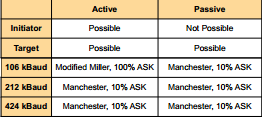
\includegraphics{moredetails.png}

\textbf{Manchester coding:} low to high 0, high to low 1. \textbf{Modified Miller coding:} low to high 0 after 0, high to high, 0 after 1, high to low 1 after 0/1. \textbf{NFC Security:} Eavesdropping/Data Modification/Replay attacks - no protection so use Secure Channel, Man in the Middle Attack -sender checks/detects disturbance and stops protocol and attacker cannot send to receiver with sender RF field on so use active/passive connection 106 kBaud. 

\section{Bluetooth 4.0: Low Energy}

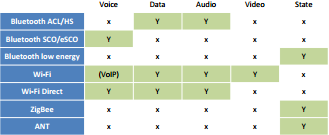
\includegraphics{srwaa.png}

WiFi Direct can support video. WiFi state inefficient. State is low bandwidth/latency/power data.\textbf{ Traditional Bluetooth} connection oriented so link maintained even when no data flowing. Sniff modes allow devices to sleep for reducing power consumption giving months of battery life and peak transmit current around 25mA. Lower power than other radio standards but not low enough power for coin cells and energy harvesting applications.\textbf{ Bluetooth low energy} is new/open/short range radio technology thats blank paper sheet design and different to Bluetooth classic(BR/EDR) optimized for ultra low power and enables coin cell battery with 20mA/5uA peak/average current. Everything \textbf{optimized} for lowest power consumption so short packets reduce transmission peak current and receive time, less RF channels improve discovery/connection time, simple state machine, single protocol, etc...\textbf{ Data throughput }not a meaningful parameter since LE doesn't support streaming, 1Mbps data rate but not optimized for file transfer, designed for sending data small discrete chunks(exposing state) triggered by local events where data read at any time by client, simple interface model(GATT). 

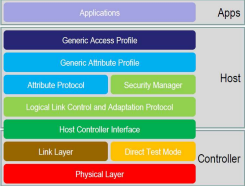
\includegraphics{blearchitecture.png}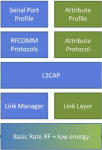
\includegraphics{dualmodestack.png}

\textbf{Dual Mode:} Bluetooth BR/EDR and LE used anywhere BR/EDR used, Single Mode implements only Bluetooth low energy so used in
new devices/applications. \textbf{Physical Layer:} 2.4GHz ISM band using 1Mbps Gaussian Frequency Shift Keying(GFSK) with larger modulation index than Bluetooth BR(better range) on 40 Channels with 2MHz spacing, $f=2402+2k$ MHz. Physical Channels with 3/37 advertising/data avoiding 802.11 channels(9 LL data channels still available).

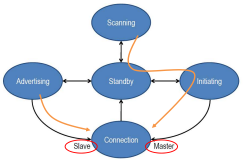
\includegraphics{llstatemachine.png}

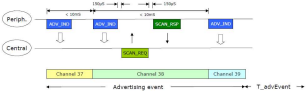
\includegraphics{advertising.png}

\textbf{Devices advertise }to broadcast promiscuously, transmit signed data to previously bonded device, advertise presence to device wanting connection, reconnect asynchronously due to local event.

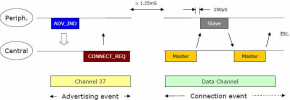
\includegraphics{datatransaction.png}

\textbf{Data transactions:} Once connection made where master informs slave hopping sequence and wake time, all subsequent transactions performed in 37 data channels, can encrypt transactions, both sleep between transactions. 

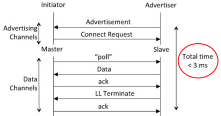
\includegraphics{latency.png}

\textbf{Battery} will costs more than electronics so sensor could run on scavenged power. \textbf{Use Cases:} Proximity, Time, Emergency, Network availability, Personal User Interface, Simple remote control, Browse over Bluetooth, Temperature Sensor, Humidity Sensor, HVAC, Generic I/O (automation), Battery status, Heart rate monitor, Physical activity monitor, Blood glucose monitor, Cycling sensors, Pulse Oximeter, Body thermometer. Everyday objects become sensors and monitor unobtrusively. Power consumption: LE $<$ Zigbee $<$ BR/EDR.

\section{Energy of Wireless Devices}

Need \textbf{long lifetime} with battery operation with no infrastructure and high deployment/replenishment costs. Continual improvement in functionality/size/weight/power at 1.6 times/year in DSP power and sensing/RF components based on MEMs but wirelessly transport bits constant energy(Shannon, Maxwell) and fundamental ADC speed$*$resolution$/$power limit so no battery technology Moore’s law for battery technology(5$\%$/year).\textbf{ Reduce energy consumption} approaches include OS turns off useless computer (IO devices like display) and application program uses less energy possibly degrading user experience quality.\textbf{ Hardware Issues:} Battery – handheld devices have disposable batteries while laptop have rechargeable batteries, Multiple power states for CPU/memory/IO - sleeping/hibernating/off, Transition between power states - Idle a time then transition into lower power state and activated when accessed. \textbf{OS Issues: }track different devices states, choose device to transition into low-power state, Window's Advanced Configuration and Power(ACPI) Interface, OS commands device driver to report states(power information) where there's overhead delay to restart device or wasted energy by unused device. \textbf{Display Energy Management:} biggest energy consumption since require backlit for bright sharp image, solutions are shut down display if no activity for some time or divide screen into zones and turn on zones with active window or change color mapping scheme. \textbf{Disk} takes substantial energy spinning at high speed even without accesses,  solutions are spin disk down after certain idle time then spin up when needed or disk cache in RAM or keep application programs informed when disk down. \textbf{Memory}: flushed cache then switch off (hibernation) so CPU has to shut off and load memory from ROM which is high overhead but might be worth while for long idle times, multiple power mode like active/nap/standby/power-down. \textbf{Wireless communications} major energy hog where energy/bit plus energy/op large even for short ranges $E_{bit}=\alpha+\beta{d^n}$ where $\alpha$ digital processing static power, $\beta$ power amp for receiver sensitivity. \textbf{Transmission energy} has heavy tails so rather have back-to-back transmissions. \textbf{Radio Electronic Trends:} move functionality from analog to digital electronics that benefit most from technology improvements, analog bottleneck but digital complexity increasing due to robustness. Either reduce energy/bit or increase energy availability. \textbf{Radio Energy Management:} interest parameter is energy consumption per bit $E_{bit}=\frac{P}{T_{bit}}$ where modulation scales with few bits/symbol and code scales with more heavy codes. \textbf{Reduced Path Loss} via Directional Antenna: smart antenna processes signals by beamforming with low/high transient/quiescent cost and reconfigurable antennas have Mechanical articulation and electrical reconfiguration with high/low transient/quiescent cost. \textbf{Exploiting Articulation and Mobility for Energy:} system lifetime improvement rich source with articulated appendaged nodes and mobile nodes controlled/predictable/unpredictable/restricted/unrestricted, opportunities for better communication and channel sensing and diversity gain due to mobility and bits/energy mechanical transport and better energy harvesting, challenges are Platforms with articulation/mobility and protocols/collaboration algorithms to exploit mobility and Understanding fundamental mobility impact on lifetime. Communication vs. Articulation has 51 degrees/second latency with Breakeven point at bits number vs. SNR gain for spending upfront energy to save on subsequent per-packet energy. \textbf{MAC energy scaling} use radios with scalable modulation/coding and MAC protocol decides which node transmits what packet at what time on what channel with what RF power with what modulation/coding setting. Radio modes include active/idle/shutdown/transient where transient period has negligible active/idle to sleep but considerable sleep to active/idle period since PLL in frequency synthesizer takes time to settle so $P_{tr} = 2P_{syn}$ and $T_{ON}$ $O(10)-O(100)$ us where mixer/power amp startup ignored but $T_{ON}$  significant packet duration fraction so packet sizes small in sensor nets for reporting events leading to high energy per bit so want fast start-up/acquisition radios. \textbf{On-demand data-driven wakeup} duty cycle radio so trade-off between energy/latency, wake-up circuit and protocols exploiting them instantly wakes up needed remote receiver radio while minimize spurious wake-ups/interference by matching destination address and preamble with cheap directional antennas. \textbf{Network energy aware routing} maximizes network lifetime since communication expensive where variances include shortest-hop (fewest nodes involved)/lowest energy route/ route via highest available energy/distribute energy burden evenly/lowest routing overhead, distributed algorithms and changing component state costs energy so use stateless routing. \textbf{Beyond Reduction by Energy Harvesting: }sensor nodes extract energy from environment and store in capacitor/battery using wind/solar/vibration/motion/chemical, challenge in managing energy harvesting with varying harvesting opportunities and extracting maximum performance, harvesting-aware network-level tasks aware of battery status and harvesting opportunities so richer nodes take more load and checking battery status not enough but learn energy environment.

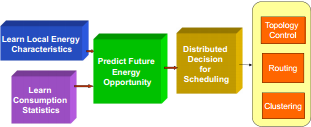
\includegraphics{harvestingaware.png}

Summary: Energy efficient radios – efficient shutdown and wake up for short range and energy performance scalability for long range, Directional antennas - directional elements electrical/mechanical reconfiguration, Exploit mobility/articulation with platforms/algorithms – better communication and channel sensing with mobility diversity gain and bits/energy mechanical transport with better energy harvesting, Energy harvesting -network operation spatio temporal characteristics aware of environmental energy availability. Challenges: Technologies – energy efficient/scalable components in radios/reconfigurable antennas/sensor processing(image, biochem) with energy harvesting wind/solar/motion/vibration/chemical and ad hoc infrastructure elements/hierarchy like energy/data mule and mobile microservers with EM and wired energy delivery, Techniques – energy/latency/accuracy/coverage trade offs with energy efficient and battery/harvesting aware algorithms and distributed in network processing, energy metrics for sensing/signal processing/event detection/communication protocols and representative functions benchmark suite and simulators with energy producers/consumers models and instrumented testbeds. Beyond Saving Energy: ambient backscatter and wireless charging.

\section{Cellular Networks}

\subsection{introduction}

Forward voice channel(FVC), Reverse voice channel(RVC), Forward control channel(FCC), Reverse control channel(RCC). Challenge is limited spectrum allocation (government regulation) so single high-powered transmitter has good coverage but frequency reuse impossible due to interference. 1960s-1970s Bell Labs developed cellular concept developed with areas divided into cells in system approach without major technological changes. Few hundred meters in cities to 10km in country each served by base station with lower power transmitter and gets total channel number portion and neighboring cells assigned different channel groups so interference minimized. \textbf{Cell shape} needs equal area without overlap between cells so choices are square/triangle/circle but for given radius hexagon provides maximum coverage area so fewest cells covers geographic region but actual cellular footprint determined by transmitting antenna contour. \textbf{Cellular Network Architecture:} Cell - covers geographic region with mobile users attach to network through base station(BS) analogous to 802.11 AP by air interface with physical/link layer protocol between mobile/BS, Mobile Switching Center(MSC) – can be mesh that connects cells to wide area network and manages call setup and mobility. \textbf{Ingredients: }mobile phones/PDAs(visible but smallest network part), antennas(still visible), infrastructure like BS/cabling/microwave links/management/databases/switching unuts/monitoring(invisible but comprise major network part). 4G different from 2/3G.

\textbf{Telephone call to mobile user:} 1 – incoming telephone call to mobile received at MSC, 2 – MSC dispatches request to all base stations in cellular system(MSCs now dispatches according to mobility patterns), 3 – base stations broadcast Mobile Identification Number(MIN)(telephone number) paging over FCC throughout cellular system, 4 – mobile receives paging message and responds identifying itself over reverse control channel, 5 – base station relays acknowledgement sent by mobile and informs MSC of handshake, 6 – MSC instructs base station to move the to issued voice channel within cell, 7 – base station signals mobile to change frequencies to unused forward/reverse voice channel pair and data message(alert) transmitted over forward voice channel to ring mobile.

\textbf{Telephone Call Placed by Mobile: }1 – mobile sends base station telephone number(MIN)/electronic serial number(ESN)/called telephone number/station class mark (SCM) which indicates the
maximum power level for user, 2 – base station relays data to MSC, 3 – MSC validates request and connects to called party through PSTN and validates base station and mobile user to move to unused forward/reverse channel pair.

\textbf{Roaming}: cellular systems allow subscriber operation in service areas other than one from which service subscribed so when mobile enters geographic area different from home service area it registered as roamer, Registration – MSC polls unregistered mobiles which respond with MINs then MSC queries mobile home for billing info, Calls – MSC controls call and bills mobile home.

\subsection{Frequency Reuse}

Sharing mobile-to-BS radio spectrum with FDMA/TDMA and CDMA. Adjacent cells assigned different frequencies avoids interference/crosstalk so reuse frequency in nearby cells with 10-50 frequencies assigned each cell and transmission. Power controlled to limit power escaping to adjacent cells so determine how many cells intervene between two same-frequency cells. \textbf{Calculation:} Each cell allocated $k$ channels and cluster has $N\in\{4,7,12\}$ cells with unique/disjoint channels so total duplex channel number $S = kN$ and cluster repeated $M$ times in system so total channel number(capacity) $C = MkN = MS$. Little’s Theorem: users in system $=$ arrival rate $*$ service time. Kendall Notation $A$(inter-arrival time distribution)/$B$(service time distribution)/$c$(server number)/$K$(system queue capacity)/$m$(customers number in source)/$Z$(queue organization), $K/m/Z$ omitted if queue/source infinite and queue FIFO, $M$ exponential distribution/$D$ discrete/$G$ general. $M/M/c/c$ queue has Poisson arrival with exponential distributed service time and $c$ servers with buffer size $c$ and blocking probability $\frac{\alpha^c}{c!\sum_{i=0\dots{c}}\frac{\alpha^i}{i!}}$ where $\alpha$ is offered load. 

\subsubsection{Cell-Size Tradeoff}

Smaller cells means higher $M$ and $C$ so channel reuse means higher capacity ans lower mobile power requirements but additional base stations required with more frequent handoffs and greater hot spot chance. Channels unique in same cluster repeated over clusters, keeping cell size same with large $N$ means weaker interference but lower capacity while small $N$ means higher capacity but more interference need for certain S/I level, \textbf{frequency reuse factor} $\frac{1}{N}$ since each cell within cluster assigned $\frac{1}{N}$ of total available channels. Connecting without gaps between adjacent cells (tessellate) need $N=i^2+ij+j^2$ where $i$ and $j$ non-negative integers. \textbf{Nearest co-channel neighbor} is $i$ cells along any chain/hexagon then turn 60 degrees counterclockwise and move $j$ cells.

\subsection{Channel Assignment Strategies}

\textbf{Fixed Channel Assignments:} each cell allocated predetermined voice channels set, if all channels cell are occupied then call blocked and subscriber not served, variation includes a borrowing strategy where cells borrow channels from neighboring cell if own channels occupied supervised by MSC. \textbf{Dynamic Channel Assignments:} voice channels not allocated permanently so each call request need serving base station requests channel from MSC which allocates channel to requested call based on decision algorithm taking into account different factors like frequency re-use and cost, more complex(real time) but reduces blocking likelihood. \textbf{Interference} major limiting factor in cellular radio system performance, co/adjacent channel interference, effects are cross talk on voice and missed/blocked calls on control and corrupts/loses data on data, interference sources are other mobiles in same cell(adjacent) or call in neighboring cell(adjacent) or other base stations operating in same frequency band(co) or non-cellular system leaking energy into the cellular frequency band(adjacent).

\textbf{Co-Channel Interference: }co-channel cells use same frequency set interference, co-channel reuse ratio $Q=\frac{D}{R}=\sqrt{N}$ where $R$  cell radius and $D$ distance between nearest co-channel cells so small $Q$ means small cluster size $N$ and large capacity while large $Q$ means good transmission quality so cellular design tradeoff, signal interference ratio(SIR, S/I) for mobile receiver $\frac{S}{\sum_{i=1\dots{i_0}}I_i}$ where $S$ is signal power from designated base station and $I_i$ is interference power caused by $i$th interfering co-channel cell. For any given antenna(BS) power at a distance $d$ is $Pr=Po(\frac{d}{do})^{-\alpha}$ where $\alpha$ is path loss exponent so $\frac{S}{I}=\frac{R^{-\alpha}}{\sum_{i=1\dots{i_0}}D^{-\alpha}_i}$. If mobile at cell center $D_i=D$ so $\frac{S}{I}=\frac{R^{-\alpha}}{D^{-\alpha}\sum_{i=1\dots{i_0}}1}=\frac{(\frac{R}{D})^{-\alpha}}{i_0}=\frac{\sqrt{3N}^\alpha}{i_0}$ for hexagon geometry. \textbf{Worst case interference} when mobile at cell boundary and experiences worst case co-channel interference on forward channel $\frac{S}{I}=\frac{R^{-\alpha}}{2(D-R)^{-\alpha}+2(D+R)^{-\alpha}+2D^{-\alpha}}$ when $i_0=6$.

\textbf{Adjacent Channel Interference }result from adjacent frequency signals to desired signal due to imperfect receiver filters allowing nearby frequencies to leak into pass band, minimized by careful filtering/assignments and keeping frequency separation between channel in cell as large as possible to reduce adjacent channel interference considerably.

\subsection{Techniques to Increase Capacity}

Wireless service demand increases cause channels assigned not enough to support required users so increase channels per unit coverage area. Approaches: \textbf{Frequency borrowing} – frequencies taken from adjacent cells by congested cells, \textbf{Cell splitting} – cells in high usage areas split into smaller cells, \textbf{Cell sectoring} – cells divided into wedge-shaped sectors each with own channel set, Microcells – antennas move to buildings/hills/lamp posts. Cell Splitting subdivide congested cell into smaller cells each with own base station so reduces antenna/transmitter power so more cells/clusters means higher capacity thus achieves capacity improvement by rescaling system. Sectoring replace single omni-directional antenna at base station with several directional antennas each radiating within specified sector thus achieves capacity improvement by rescaling system with less co-channel interference so cells number in cluster can be reduced and larger frequency reuse factor and capacity.\textbf{ Micro Cell Zone} Concept has large control base station replaced by several lower powered transmitters on cell edge so mobile retains same channel and base station switches channel to different zone site as mobile moves across zones, since channel active only particular zone in which mobile traveling base station radiation localized and interference reduced. \textbf{Offloading Cellular Traffic:} explosive cellular traffic growth means highly dynamic traffic and large peak-to-average traffic ratio so provision based on peak load too costly thus cellular provider purchase bandwidth on demand from 3rd party resources that gain additional revenue and achieve significant savings to improve user experience but need incentive framework for collaboration. \textbf{Dynamic Spectrum Auction:} buy/sell spectrum among cellular providers, fundamentally different from traditional auction since spectrum reused and wireless interference complicates competition. Cellular efficiency decreases with more cells without reuse.

\subsection{Handoff}

Mobile moves into different cell while conversation in progress so MSC automatically transfers call to new channel belonging to new base station, important task in any cellular radio system and must be performed successfully/infrequently/imperceptible to users, identify new base station and channel allocation in new base station with higher priority than initiation request. \textbf{Types}: Intra-cell, Inter-cell and Intra-BSC, Inter-BSC and Intra-MSC, Inter-MSC. Base Station Control(BSC) handles multiple base stations, MSC handles many BSCs.  \textbf{Margin Choice:} $\Delta$ call minimum acceptable signal, too small means insufficient handoff time so more call losses, too large means too many handoffs so MSC burden. Styles: \textbf{Network Controlled Handoff(NCHO)} - first generation cellular system where each base station constantly monitors signal strength from mobiles and MSC decides if handoff necessary based on measures so mobile passive and MSC burden,\textbf{ Mobile Assisted Handoff(MAHO)} – second generation systems where mobile measures received power from  base stations and report to serving base station and handoff initiated when power received from neighboring cell exceeds current value by certain level or time period which is faster since measurements made by mobiles no MSC monitor signal strength, Mobile Controlled Handoffs. Types: \textbf{Hard handoff} - FDMA/TDMA where mobile has radio link with one BS at anytime so old BS connection terminated before new BS connection made, \textbf{Soft handoff} – CDMA systems where mobile has simultaneous radio link with BSs at any time so new BS connection made before old BS connection broken and mobile unit remains in this state until one base station clearly predominates.

\section{Network Security Overview}

Network security princicples: cryptography beyond confidentiality, authentication, message integrity.

\subsection{Network Security}

\textbf{Confidentiality} - sender receiver understand message contents so sender encrypts message and receiver decrypts message, Authentication - sender receiver confirm each other's identity,\textbf{ Message integrity} - sender receiver ensure message not altered in transit or afterwards without detection, \textbf{Access and availability} - services accessible/available to users. Intruder intercept(eavesdrop)/delete/add(insert)/impersonation(spoof packet fields)/hijacking( take over ongoing connection by removing sender/receiver and inserting itself)/denial of service(prevent service from being used) messages. Sender/receiver are people, browser/server for electronic transactions, on-line banking client/server, DNS servers, routers exchanging routing table updates, cell phones, RFID tags, NFC device, sensors, etc...

\subsection{Principles of Cryptography}

\textbf{Substitution cipher} substitutes one thing for another, \textbf{monoalphabetic} cipher substitutes one letter for another where key is 26 letters to 26 letters mapping. \textbf{Polyalphabetic} encryption has $n$ monoalphabetic cyphers $M_1,M_2\dots,M_n$ with each new plaintext symbol using subsequent monoalphabetic pattern in cyclic pattern where key $n$ ciphers and cyclic pattern. \textbf{Breaking encryption scheme}: Cipher text only attack - intruder analyze by search through all keys which must be able to differentiate plaintext from gibberish or statistical analysis, \textbf{Known plaintext attack} - intruder has some plaintext corresponding to some ciphertext, \textbf{Chosen plaintext attack} - intruder can get the cyphertext for some chosen plaintext. \textbf{Cryptography Types}: uses secret keys with public algorithm, public key cryptography involves two keys while symmetric key cryptographyi involves one key, hash functions involves no keys.

\textbf{Symmetric Ciphers}: stream ciphers encrypt one bit at time while block ciphers break plaintext message in equal-size blocks and encrypt block as unit. Stream ciphers combine each keystream bit with plaintext bit to get ciphertext $c(i)=ks(i)\oplus{m(i)}$ and $m(i)=ks(i)\oplus{c(i)}$ where $m(i)/ks(i)/c(i)$ is $i$th bit of message/keystream/ciphertext. RC4 Stream Cipher extensively analyzed and considered good with 1-256 byte key used in WEP(isn't secure). Block ciphers process messages $k$ bit blocks with $k$-bit plaintext block to k-bit ciphertext block 1-to-1 mapping.  $2^k!$ mappings so table too big so use function that simulates randomly permuted table. Single round input bit limitly affects output bits so use $n$ rounds but becomes less efficient as $n$ increase. Breaking message in $k$-bit blocks and encrypting separately cause same plaintext block give same cyphertext so enerate random $k$-bit number $r(i)$ for each plaintext block $m(i)$ for $c(i)=K_S(m(i)\oplus{r(i)})$ and $m(i)=K_S(c(i))\oplus{r(i)}$ but inefficient since need to send $c(i)$ and $r(i)$. Cipher Block Chaining(CBC) generates own random numbers and encrypt current block wit hprevious block result $c(i)=K_S(m(i)\oplus{c(i-1)})$ and $m(i)=K_S(c(i))\oplus{c(i-1)}$, encrypt first block with random public block initialization vector(IV) $c(0)$ changed for each message/session which guarantees different ciphertext on same message. Data Encryption Standard(DES) US standard with 56-bit symmetric key and 64-bit plaintext input using cipher block chaining but phrase brute force decrypted in less than a day and no known good analytic attack so make DES more secure with 3DES that encrypts 3 times with 3 different keys, operate by initial permutationthen 16 identical function application rounds using different 48 bits of key then final permutation. Advanced Encryption Standard(AES) new symmetric-key NIST standard replacing DES that processes data in 128 bit blocks amd 128/192/256 bit keys while brute force decryption take DES 1s takes AES 149 trillion years.

\textbf{Public Key Cryptography}: sender/receiver do not share secret key with public encryption key $K^+$ known to all and private decryption key $K^-$ known only to receiver and need $K^-(K^+(m))=m$ and impossible to compute $K^-$ from $K^+$. Modular arithmetic - $x$ mod $n$ is $x$ remainder when divide by $n$ and $[(a$ mod $n)+(b$ mod $n)]$ mod $n=(a+b)$ mod $n$, $[(a$ mod $n)-(b$ mod $n)]$ mod $n=(a-b)$ mod $n$, $[(a$ mod $n)*(b$ mod $n)]$ mod $n=(a*b)$ mod $n$ so $(a$ mod $n)^d$ mod $n=a^d$ mod $n$. Rivest Shamir Adleman: message is bit pattern uniquely represented by integer number thus encrypting message is encrypting number,  Creating public/private key pair- choose two large prime numbers $p,q$ and compute $n=pq,z =(p-1)(q-1)$ and choose $e<n$ relatively prime with z and choose $d$ such that $ed$ mod $z=1$ so public key is $(n,e)$ and  private key is $(n,d)$, encrypt message $m<n$ by $c=m^e$ mod $n$ and decrypt $m=c^d$ mod $n$, for any $x,y$ $x^y$ mod $n =x^{(y\textit{ mod }z)}$ mod $n$ where $n=pq$ and $z=(p-1)(q-1)$ thus $c^d$ mod $n=(m^e$ mod $n)^d$ mod $n=m^{ed}$ mod $n=m^{(ed\textit{ mod }z)}$ mod $n=m^1$ mod $n=m$, $K^-(K^+(m))=m=K^+(K^-(m))$ since $(m^e$ mod $n)^d$ mod $n=m^{ed}$ mod $n=m^{de}$ mod $n=(m^d$ mod $n)^e$ mod $n$, knowing public key $(n,e)$ find factors of $n$ to determine $d$ without knowing factors $p$ and $q$ which is hard, generate RSA keys by making good guess then apply testing rules. $5.57\%$ TLS hosts and $9.60\%$ SSH hosts use repeated keys in vulnerable manner, can obtain RSA private keys for $0.50\%$ TLS hosts and $0.03\%$ SSH hosts since their public keys shared nontrivial
common factors due to entropy problems. Asymmetric crypto expensive( DES 100 times faster than RSA) but simplify key exchange while symmetric crypto cheap but need to establish key so exchange symmetric session key using RSA then use symmetric key cryptography. 

\subsection{Message Integrity}

Allows communicating parties verify received messages authentic the message content not altered from expected message source and message not replayed and message sequence maintained.

\textbf{Message Digests}: many-t-1 has function $H$ takes arbitrary message and outputs fixed-length string message signature, desirable properties are calculation ease/irreversibility(can’t determine $m$ from $H(m)$)/collision resistance(computationally difficult to produce $m,m’$ such that $H(m)=H(m’)$)/random output. Internet checksum poor message digest since many-to-one produces 16-bit sum of input but not collision resistant. MD5 hash function computes 128-bit message digest in 4-step process., SHA-1 US standard 160-bit message digest. 

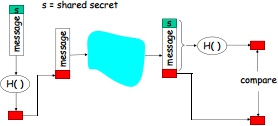
\includegraphics{mac.png}

\textbf{Message Authentication Code(MAC)}: keyed hash authenticates sender and verifies message integrity without encryption $MD_m = H(s||m)$ and send $m||MD_m$. HMAC - addresses subtle append security flaws by prepending secret to message and hashing and prepending secret to digest hashing. End-point authentication ensures message originator against playback attack using nonce $F$ in $MAC=H(m,s,R)$.

\textbf{Digital Signatures:} sender digitally signs document with private key, establishing is owner/creator similar MAC but use public-key cryptography, verifiable/nonforgeable since recipient can prove no one else signed document, singed message digest.

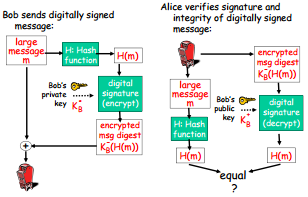
\includegraphics{ds.png}

\textbf{Certification Authorities(CA): }binds public key to entity $E$(person, router) that registers public key with CA identity proof then CA creates certificate binding $E$ to public key that contains $E$'s public key digitally signed by CA. Primary standard X.509 contains issuer name/entity information/Entity public key/digital signature(with issuer’s private key), Public-Key Infrastructure(PKI) -certificates and certification authorities considered heavy.

\section{Insecurity of 802.11}

\textbf{Wired Equivalent Privacy(WEP)} wireless standard 802.11 link layer failed confidentiality(prevent eavesdropping)/access control(prevent unauthorized access)/data integrity(prevent message tampering). 1987 Ron Rivest Cipher 4(RC4) encryption used in SSL/WEP $m||CRC(m)\oplus{RC4(k,IV)}=C$ then prepend IV, decryption $C\oplus{RC4(k,IV)}=m||CRC(m)$. Two ciphers $C_1,C_2$ using same $RC4(v,k)$ has $C_1\oplus{C_2}=P_1\oplus{P_2}$ which needs ciphertexts reusing keystream and plaintexts partial knowledge to succeed attack. Shared key $k$ changes rarely so public IV reuse causes keystream reuse. \textbf{IV Usage:} 24 bits inherent limit so busy 5Mbps access point 11 hours exhaust available space and common practices make IV reuse more often with random IV selection so birthday paradox(5000 packets needed to find collision) and common PCMCIA cards sets IV zero then increment 1 each packet so keystreams of low-valued IVs reused many times and tandard recommends not requires IV change on every packet. \textbf{Exploiting}: one message plaintext known then other immediately obtainable and known techniques for breaking reused keystreams and as reused keystream increases breaking them becomes easier, trial/error since many IP traffic fields predictable. or send known text and sniff encrypted text since AP broadcast both encrypted/unencrypted form when subnet has both WEP/non-WEP clients, store keystream in 24GB decryption dictionary after plaintext obtained and dictionary size independent of key size. \textbf{Consequences}: Message Modification - CRC32 checksum and RC4 message linear function so distributes over XOR operation $C(x\oplus{y})=C(x)\oplus{C(y)}$ so given $C$ create $C'$ that decrypts to $M'$ instead of $M$ by $C\oplus{\Delta||CRC(\Delta)}=(RC4(k,IV)\oplus{m||CRC(m)})\oplus{\Delta||CRC(\Delta)} = RC4(k,IV)\oplus({m||CRC(m)}\oplus{\Delta||CRC(\Delta)})= RC4(k,IV)\oplus{M'||CRC(M')}$, \textbf{Message Injection} - WEP checksum unkeyed message function of so can use keystream forever $C'=M'||CRC(M')\oplus{RC4(IV,k)}$ and reuse old IV values without triggering receiver alarms. \textbf{Weakness}: linear RC4 efficient but insecure and $C_1\oplus{C_2}=P_1\oplus{P_2}$ so inferring $P_1,P_2$ gets keystream by XOR plaintext with ciphertext, frequent IV reuse with inherent 24-bit limit and practical use make reuse more frequent, poor key management has key shared among many entities and rarely changed, confidentiality/access control/data integrity violated. \textbf{Countermeasure}: Improve key management so everyone has own key and revent key reuse with more secure cryptographic algorithms and end-to-end security. Security protocols design difficultso public review and combining several secure algorithms doesn't mean result secure and avoid engineering perspective dictating cryptographic algorithms selection.

\textbf{80211i}: Replace WEP for confidentiality/data origin authenticity/data integrity/replay protection, better encryption – temporal key integrity protocol(TKIP) changes temporal keys every packet but still encrypt using RC4 for WEP inter-operation AES requiring coprocessor and stronger MAC, key management – preshared key with easier setup and 802.1x.

\textbf{802.1x:} client only WLAN authentication framework with strong mutual authentication use Extensible Authentication Protocol(EAP) authenticating users, multi-provider access points shared among different service providers so each network has own SSID and 802.1x allows APs implement different policies.

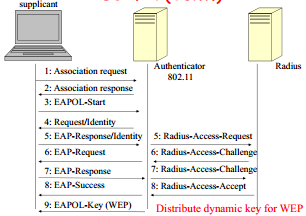
\includegraphics{8021x.png}

IEEE 802.11i/802.11x insufficient since VPN technologies (IPSEC, TLS, SSL) satisfy public/corporate domain e2e security requirements.

\section{Wireless Security: DOS Attacks and Defenses}

\subsection{Physical Layer: Jamming}

\subsubsection{Radio Interference Attack}

Intentionally interfering wireless communications \textbf{physical} transmission/reception by emitting radio frequency signals not under MAC protocol, mitigate jamming with spread spectrum. \textbf{Attack Models:} Constant – always emit random radio signal bits, Deceptive - always emit preamble bits, Random - alternate between sleeping/jamming states to conserve energy, Reactive - transmit signal when jammer senses channel activity so harder detection. Packet Send/Delivery Ratio(PSR/PDR). 

\subsubsection{Measurements to Detect}

\textbf{Signal Strength }- match jam signals with legitimate signal pattern, \textbf{Carrier Sensing Time }- jamming incurs long carrier sensing time, \textbf{PDR} - jamming incurs lower PDR. Signal strength spectral discrimination employed Higher Order Crossings (HOC) to differentiate between samples. Small PDR degradation means normal congestion while large PDR degradation mans sender battery failure or out of communication range or jammed, better measure than signal strength or carrier sensing time if can differentiate jamming attack from other network dynamics but not enough alone.

\subsubsection{Detection Schemes}

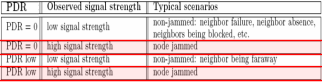
\includegraphics{pdrss.png}

PDR classify poor link and signal strength reactive consistency check with jammed region $SS>-73$ dBm and $PDR<65\%$. Disadvantage - PDR window jammed for a while and hard to choose SS granularity with mobility. PDR classify poor link and coordinate proactive consistency check fails with isolated nodes and obstacles, network density and location advertisement frequency matters. These heuristics fail sometimes.

\subsection{MAC Layer: Greedy MAC}

\subsubsection{Data Plane}

Hotspot industry tremendous financial success increases user misbehave motives. More effective than routing/transport misbehavior since MAC misbehavior applicable to WLAN and multihop wireless networks affecting all traffic using same MAC and further combined with other misbehavior. \textbf{System Model:} AP trusted and implements detection system without client modification, clients greedily misbehave but not maliciously disrupt network.\textbf{ Misbehavior Techniques:} scramble CTS/DATA/ACK frame artificially increases CW or transmit RTS/DATA SIFS or increasing NAV or reduce backoff time, combining several techniques or dynamically changing misbehavior.\textbf{ Detect misbehavior} without throughput since affected by many factors like traffic demands/SNR/transport protocol/device drivers/protocol implementation/etc... so backoff most direct cheater detecter but determine backoff time and hidden terminals since not everyone sees idle/busy channels simultaneously, MAC can have CRC with each part of packet, multiple antennas mitigate interference. \textbf{Domino}: Collect traffic traces of sending stations every monitoring periods and test traces for fewer retransmissions(scrambles), shorter DIFS and oversized NAV(manipulated protocol), maximum/actual/consecutive backoff(small CW) but cheater can exploit cheat$\_$count decrementation by cheating every other time. \textbf{Simulation Impact:} cheater gains significant throughput than well-behaved stations and Domino accurately detects backoff interval under UDP traffic, MAC misbehavior serious and easy since IEEE 802.11 standard complaint without hardware change.

\subsubsection{Control Plane}

\textbf{Misbehavior Techniques:} spoof disassociation/deauthentication frames since neither authenticated, screw power control by spoof polling message causing AP discard client packet while sleeping or spoof TIM message convincing client of no pending data or spoof beacon frames with incorrect timestamp screwing client/AP synchronization since management frames not authenticated.

\subsection{Network Layer: Routing Attacks}

\textbf{Ad hoc network routing protocol} assume every node cooperates and follows protocol, DSR focus without optimization and model attacks and present on-demand secure ad hoc network routing protocol design/evaluation(Ariadne with TESLA). 

\textbf{Assumptions}: Network - network layer attack and bidirectional links may drop/corrupt/reorder/duplicate packets in transmission, Node - little computational resources and loosely synchronized with TESLA and GPS can be used but trusted tamper proof hardware, Ariadne relies on key secrecy/authenticity mechanism like pair wise shared secret keys or TESLA that assumes key sharing mechanism between communicating nodes with each node one authentic public TESLA key or digital signature with each node one authentic public key.

\textbf{Routing Security:} Attacker Model - omit passive attacks on confidentiality/anonymity for active-$y$-$x$ model where attacker has $x$ nodes with $y$ nodes compromised nodes and distribute cryptographic information to $x-y$ nodes or active VC model where attacker has nodes in vertex cut bith target authentication/routing, General Attacks - routing disruption attacks by dysfunctional routing with loop/black hole/gray hole/detours/gratuitous detour/black mail/worm hole or rushing attack by disseminating route request packet quickly to suppress later legitimate route requests or resource consumption attacks by consuming bandwidth/computational resource or inject extra packets or DoS effective for flooded control packets.

\textbf{Goals}: target/data authenticate nodes with TESLA and shared symmetric key since route reply has MAC list of all route nodes or digital signature since route reply packet has signature list and per-hop hashing verify  no hop omitted/added

\textbf{TESLA}: assymmetric broadcast authentication protocol with single (MAC) using clock synchronization and delayed key disclosure instead of one-way expensive trapdoor functions so assumes loose time synchronization and known pessimistic end-to-end delay with maximum synchronization error $\Delta$ and pessimistic end-to-end delay $\epsilon$ and key publishing delay $d$. Generate one-way hash chain $K_n,\dots,K_0\ni{H(K_i)=K_{i-1}}$ and publish $K_i$ at $T_0+it_p$ and send $P_i=(M_i||MAC(K_i, M_i)||K_{i-d})$ or $P_t$, drop $P_i$ if ${T_s+\epsilon+2\Delta}\leq{T_r}<T_0+it_p$ else verify $K_n=H^{n-i}(K_i)$ and compute $MAC(K_i,M_i)$ with $K_i$ in $P_{i+d}$, TESLA verifies messages in next time interval. 

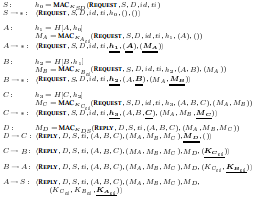
\includegraphics{ariadnerreq.png}

\textbf{Ariadne}: Design Goals - low computational/communicational overhead to prevent DoS while using TESLA for authenticating routing path nodes. \textbf{Maintenance} - $(RE||B,D||t_i||MAC_{K_{B_{ti}}}(RE||B,D||t_i)||K_{B_{t_{i-d}}})$ and $(RE||B,D||t_{i+d}||MAC_{K_{B_{t_{i+d}}}}(RE||B,D||t_{i+d})||K_{B_{t_i}})$. \textbf{Evaluation} - moves to random way point model and guarantees destination return route reply with compromised neighbors then route along uncompromised route while Preventing attacks with MAC hop-by-hop hashing and TESLA maximum end-to-end delay and hash-chaining feature and generates less packets and latency than unoptimized DSR since it delays with more stable routes which mitigates route flapping. 

\subsection{Transport Layer: Cross layer Attacks}

Attackers prevent legitimate users from getting served commonly by effectively manipulating lots of traffic upper layer protocols regardless but easy to detection.

\textbf{Black Holes(BH):} participate routing control operations to establish routes through themselves then drop all data packets, detect by watch next hop but dynamic power control/directional antennas/asymmetric links have false positives(heard by next hop but not previous hop) and false negatives(heard by previous hop but not next hop) or choose detection timescales where large packet losses needs more affected traffic.

Attract more affect traffic with \textbf{rushing attacks} getting twice as many flows compared with uniform graph drops goodput drops $52\%$ - $34\%$ with $10\%$ attackers or mobile attackers attain optimal position that affects large flow amount.

\textbf{Jellyfish(JF):} manipulating small traffic amount so harder to detect, cross-layer attack exploit feedback-based protocol (TCP) by reorder/periodic dropping/delay variance attacks. \textbf{Reorder Attack deliver} all packets randomizing in FIFO buffer which results in near-zero goodput despite delivering all packets and more severe for more hops and hard to detect because no packet dropping. \textbf{Periodic dropping} all packets for short time period per retransmission time-out(RTO) has consecutive packet losses means TCP timeout and drop again RTO seconds later, hard to detect since dropping small packet fraction, drops packets 90ms every second(dropping $9\%$, forwarding $91\%$) and dard to detect because imitates severe congestion. \textbf{Delay variance manipulation} by equally alternating between serving and not serving packets resulting in TCP bursty due to selfclocking thus increasing collisions/loss with incorrect available bandwidth estimations and excessively high RTO value which decreases TCP goodput. JF nearly same impact as BH nut only works for TCP flows while BH works for both TCP/UDP but JF much harder to detect than BH.

\textbf{How to react:} Once malicious nodes detected establish new path excluding node malfunctioning path but difficult small/sparse networks or employ multipath routing and adapt path weights to goodput but severely decreases TCP throughput or establish backup routes keeping all route reply messages. Open/closed loop protocol affects large/small traffic amount.

\section{Fingerprint}
\subsection{WiFi Security And Privacy}
WEP comprises confidentiality, access control, and data integrity. \textbf{Solutions?} 802.1x dynamically generates WEP key, 802.11i: better encryption, End2end security: VPN. \textbf{Best security practice:} bootstrap. Three phases: discover, authenticate and bind, send data. But \textbf{privacy problems remain.} Many exposed bits are (or can be used as) identifiers that are linked over time. Our packets leave “digital fingerprints” that reveal who we are -- And thus where we have been. \textbf{Motivation: The Mobile Wireless Landscape:} Location privacy is growing concern
. Wireless Privacy Protection Act [U.S. House Bill ‘05]
. Geographic location/privacy working group. \textbf{Under The Mobile Wireless Landscape} A well known technical problem
– Devices have unique and consistent addresses – e.g., 802.11 devices have MAC addresses. Thus, fingerprinting them is trivial! The widely proposed technical solution – Pseudonyms: Change addresses over time. \textbf{Pseudonyms are not enough}
– Implicit identifiers: identifying characteristics of traffic.E.G.,most users identified with 90 percent accuracy in hotspots. \textbf{Contributions}. Four Novel 802.11 Implicit Identifiers. Automated Identification Procedure. Evaluating Implicit Identifier Accuracy.

\subsection{Four Novel 802.11 Implicit Identifiers}
\textbf{Implicit Identifiers by Example}
. Consider one user at SIGCOMM 2004– Transferred512MBviaBitTorrent. Poor network etiquette?
– Seenina“anonymized”wirelesstrace. MAC addresses hashed, effectively a pseudonym. Can we identify the culprit using implicit identifiers? Implicit identifier:\textbf{SSIDs in probes} – Set of SSIDs in 802.11 probe requests – Many 802.11 drivers search for preferred networks – Usually networks you have associated with before. \textbf{Limitations} – Infrequent transmission. – Non unique SSID. – Preferred networks change over time. Implicit identifier:\textbf{network destinations} – IP <address, port> pairs in network traffic – At SIGCOMM, each visited by 1.15 users on average – Some nearly-unique destinations repeatedly visited (e.g., email server).– Will SSL and IPSec mask this identifier? Implicit identifier:\textbf{broadcast packet sizes} – Set of 802.11 broadcast packet sizes in network traffic – E.g., Windows machines NetBIOS naming advertisements; FileMaker and Microsoft Office advertise themselves. Implicit identifier:\textbf{MAC protocol fields}
– Header bits (e.g., power management., order)
– Supported rates
– Offered authentication algorithms. \textbf{More implicit identifiers exist} Results we present establish a lower bound. Fixing Implicit Identifiers is not Simple: 
1. Encryption does not prevent traffic analysis. Cover traffic? – Challenge: Shared medium leads to large performance hit 2. Service discovery is done in the clear. Don’t probe? – Challenge: Beaconing is often undesirable also. 3. Implementation and configuration variation. Standardize? – Challenge: Ambiguity of specifications.

\subsection{Automated Identification Procedure}

\textbf{Tracking 802.11 Users}
. Many potential tracking applications: Was user X here today? Where was user X today? What traffic is from user X? When was user X here? Etc. \textbf{Tracking scenario}: Every users changes pseudonyms every hour– Adversary monitors some locations. Thus, one hourly traffic sample from each user in each location. Build profile from training samples where first collect traffic known from user X and from random others then classifyobservation samples. \textbf{Sample Classification Algorithm}. A simple approach: naive Bayes classifier. Derive probabilistic model from training samples. Givens with features F,answer“yes”if: Pr[ s from user X $|$ s has features F ] $>$ T for a selected threshold T. F is feature set derived from implicit identifiers. Deriving features F from implicit identifiers using set similarity(Jaccard Index) weighted by frequency $s=\frac{\sum_{e\in{Profile\cap{Set_s}}}w(e)}{\sum_{e\in{Profile\cup{Set_s}}}w(e)}$ where $w(e)$ low/high when common/rare.



\subsection{Evaluating Implicit Identifier Accuracy}
\textbf{Evaluating Classification Effectiveness} Simulate tracking scenario with wireless traces: Split each trace into training and observation phases. Simulate pseudonym changes for each user X. \textbf{Question}: Is observation sample s from user X?
Evaluation metrics: 1. True positive rate(TPR): Fraction of user X’s samples classified correctly. 2. False positive rate (FPR): Fraction of other samples classified incorrectly. \textbf{Individual implicit identifiers give evidence of identity. We can identify many users in all environments. Some users much more distinguishable than others. One application: }Question:Was user X here today? More difficult to answer: Suppose N users present each hour. Over an 8 hour day, 8N opportunities to misclassify. Decide user X is here only if multiple samples are classified
as he is. Revised: Was user X here today for a few hours?
\textbf{Majority of users can be identified if active long enough. Summary:} Implicit identifiers can accurately identify users – Individual implicit identifiers give evidence of identity. – We can identify many users in all environments – Some users much more distinguishable than others. Understanding implicit identifiers is important – Pseudonyms are not enough – We establish a lower bound on their accuracy. Eliminating them poses research challenges. 

\subsection{\textbf{Other Types of Fingerprints:}} Device and software fingerprints. RF environment fingerprints. Traffic fingerprints. User fingerprints.
\textbf{Device and Software Fingerprints}
. Clock-skew fingerprints – Computer forensics – Tracking and unanonymizing anonymized traces – Rouge AP detection. Device driver fingerprints – No detailed specification of active scanning scheme. Thus different implementations. \textbf{RF Fingerprints}. RF antenna fingerprints. Radiometric signatures – Signal leakage in adjacent channels is device dependent. Wireless channel fingerprints – Key establishment is hard in mobile networks – Wireless channel between two parties is unique and decorrelates rapidly in space – Use wireless channel as key. \textbf{Traffic Fingerprints}. Identify web transfers using timing and sizes – Even though content is encrypted. Identify applications from implicit identifiers in encrypted traffic – Packet size, timing, header (if available). Timing analysis of keystrokes – SSH sends each keystroke as one message – Keys typed with alternating hands, with the same hand different fingers, with the same finger, number vs. alphabetic, lowercase or uppercase – Infer length and content. \textbf{User Fingerprints}. Click-prints – Inter click time is user specific Thus, track users. This paper – 802.11 fingerprints for individual users

\subsection{Improving Wireless Privacy with an Identifier-Free Link Layer Protocol}

\subsubsection{Motivation and Goals}
\textbf{Local service discovery (SD)} Used to find: 802.11 networks• consumer electronics• local services• other applications. \textbf{How do we perform SD?} Services send announcements and/or clients send probes (typically via unencrypted broadcast)
Important properties: Plug-and-play networking
– Can proceed automatically without user input• Disconnected operation – Requires only communication medium between client and service. \textbf{What are the disadvantages of SD?} \textbf{Problem 1: SD reveals inventory} The devices I have: Problem: “Phone pirates in seek and steal mission”. TheapplicationsIamrunning
Problem: “Apple Mac OS X mDNSResponder buffer overflow vulnerability”. \textbf{Problem 2: SD reveals identity} Announcements expose explicit identifiers: Problem: Some services are private and want to be hidden. Problem: Mobile “services” vulnerable to tracking. \textbf{Problem 3: SD reveals history} Probes can reveal services you have used. Problem: Network names can be correlated with location. (e.g., using a wardriving database). \textbf{Problem 4: SD is not authenticated} Authentication occurs only after SD – Problem: Anyone can elicit a response, even if they are not trusted to access the service. \textbf{Fundamental Problem: } Many exposed bits are (or can be used as identifiers that are linked over time. \textbf{Problem 1:} Long-term linking: Easy to identify and relate devices over time. Linking enables location tracking, user profiling, inventorying, relationship profiling, ... \textbf{Problem 2}: Short-term linking: Easy to isolate distinct packet streams. Isolated data streams are more susceptible to side- channel analysis on packet sizes and timing
– Exposes keystrokes, VoIP calls, webpages, movies, ... \textbf{Goal:} Make all bits appear random. \textbf{Chanllenge: } Filter without identifiers. (Which packets are mine?) 

\subsubsection{Design Requirements}
When A generates Message to B,she sends: PrivateMessage = F(A, B, Message) where F has these properties: – Confidentiality: Only A and B can determine Message. - Authenticity: – B can verify A created PrivateMessage. – Integrity: B can verify Message not modified. – Unlinkability: Only A and B can link PrivateMessages to same sender or receiver. – Efficiency:
B can process PrivateMessages as fast as he can receive them. 


\subsubsection{Straw man: MAC Pseudonyms}
\textbf{Idea}: change MAC address periodically – Per session or when idle• \textbf{Other fields remain} (e.g., in discovery/binding) – No mechanism for data authentication/encryption – Doesn’t hide network names during discovery or credentials during authentication• \textbf{Pseudonyms are linkable in the short-term} – Same MAC must be used for each association – Data streams still vulnerable to side-channel leaks. 

\subsubsection{Straw man: Encrypt Everything}
\textbf{Idea:} Use bootstrapped keys to encrypt everything. \textbf{Straw man: Public Key Protocol} Slow! \textbf{Straw man: Symmetric Key Protocol} Slow! Can’t identify the decryption key in the packet or else it is linkable. Different symmetric key per potential sender. 


\subsubsection{Solution: SlyFi}
• Symmetric key almost works,but tension between: – Unlinkability: can’t expose the identity of the key – Efficiency: need to identify the key to avoid trying all keys• Idea:Identifythekeyinanunlinkableway • Approach:
– Sender A and receiver B agree on tokens: $T_1^{AB}, T_2^{AB}, T_3^{AB}, ...$ – A attaches $T_i^{AB}$ to encrypted packet for B - If it doesn’t have $T_i^{AB}$: discard (efficient message filtering, use $T_i^{AB}$ to extract the corresponding key for decryption. – But how to establish $T_i^{AB}$? \textbf{SlyFi: Other Protocol Details} 1• Broadcast
– Broadcast frames encrypted using a shared
broadcast key and sequence number 2• Higher-layer binding – Bind to pseudonym addresses (e.g., ARP binds IP and link address, now Tryst binds pseudo IP)
3• Time synchronization – Encrypt timestamp info. In beacon msg. using a shared broadcast key (since only clients on the network need that info.) 4• Roaming – Use shared broadcast key (since APs are usually in the same admin domain) 5• Coexistence with 802.11 – Encapsulate SlyFi msg to management frames 6• Link-layer ACKs – Use cumulative software acks \textbf{Performance Evaluation} SlyFi implementation: – Linux kernel module using Click Modular Router – Run on Soekris devices (similar to APs, iPods, etc.)• Comparison protocols: – wifi-open: 802.11 with no security. – wifi-wpa: 802.11 with WPA PSK/CCMP – public-key: straw man. – symmetric-key: straw man – armknecht: previous header encryption proposal. \textbf{Discovery/Binding Time} SlyFi link setup has less overhead than WPA. \textbf{Data Throughput} With simulated AES hardware performs like symmetric key. 

%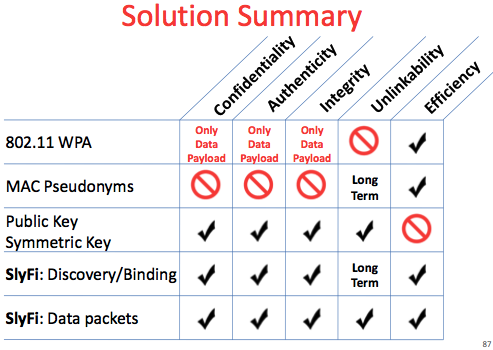
\includegraphics{solutionsummary.png}

\textbf{Conclusion}• Wireless devices are becoming personal and pervasive• Best practices do not protect users from simple attacks – Long-term linking: tracking, profiling, inventorying – Short-term linking: side-channel attacks• SlyFi makes these attacks much more difficult to do – Removes all bits that are (or can be used as) identifiers.

\section{Emergent Network}

\textbf{Wireless Communication}: Medium: Radio frequency, Light(Images, Videos), Sound. WiFi spectrum saturated so visible light is alternative like QR code. Different medium has different characteristics and poses different challenges. Light communication is directional interference-free wireless links. Vehicular/sky/minature wireless networks/apps.

\subsection{QR Code}

\textbf{1.Quick Response(QR Code)}. \textbf{UPC}1. Wallace Flint first suggested an automated checkout in 1932 2.UPC bar code formats developed in the 40’s, 50’s, 60’s. 3.Grocery Industry adopted the UPC (based on an IBM proposal) April 3, 1973. 4.With computerized scanning, inventory, With computerized scanning, inventory, UPCs are ubiquitous on every product! \textbf{What is a QR Code}. Matrix or two dimensional bar code, It is a more advanced bar coding system, Very fast readability Instant access. Eliminates the memorization of URLs. \textbf{History}. Invented by Denso wave in 1994 for tracking vehicles during manufacture. Now is one of the most popular 2-D barcode. \textbf{Applications}. URL rediction . Virtual stores. Code payment . Web login. Encryption. \textbf{Uses for QR codes} 1. Advertisements 2. Guided tours 3. Creative ice breakers 4. Packing and organization of products and shipping 5. Uses in education.\textbf{Risks}. Redirected URLs may host javascript, which can exploit vulnerabilities. QR code reader may allow use of the camera, Internet, read/write contact data, GPS, browser history, etc. In Russia, a malicious QR code caused phones that scanned it to send premium texts at a fee of US 6 each.\textbf{ Open Issues}. Increase data rates. Resilient against blurring and viewing angle– Blur: pixels bleed into each othe– Perspective distortion: squeezed or stretched. Shift from spatial to frequency domain since frequencies don't bleed into each other. Automatic rate adaptation.

\subsection{Dhwani: Peer-Peer Secure Acoustic NFC}

\textbf{Near Field Communication} (NFC). Communication between physically proximate devices. Key Advantage: No network configuration effort.Association by proximity: devices are connected to each other by virtue of proximity. Used in contactless payments, short data transfer, ticketing, healthcare etc. NFC - Limitations. Low levels of penetration of NFC hardware today. NFC standard does not define security at the physical layer. \textbf{We can enable secure NFC-like communication in today's devices} 

2.1. \textbf{Dhwani - acoustic NFC system.} Uses phone’s speaker and microphone. Software only – can be a downloadable app. Currently supports upto 2.4 Kbps data rate over 1 KHz bandwidth. 2.JamSecure – secure communication. Information-theoretic approach to security. Security at physical layer by jamming and self-interference cancellation at the receiver. 

\subsubsection{Dhwani: Acoustic NFC System}

Challenges in acoustic communication and Dhwani system design\textbf{Acoustic Communication - Challenges:} RF Communication: 1) Antenna frequency response is flat. 2) Multipath (in μs) 3) Channel is defined – interference is limited. Acoustic Communication: 1) Speaker-mic frequency selectivity 2) Echo (in ms) 3) Channel not defined – ambient noise interference. \textbf{Challenge 1 : Frequency selectivity}. Imperfect electromechanical conversion. Frequency response is not uniform. Significant degradation above 12 KHz – significant data loss in that band. \textbf{Challenge 2 : Ringing and rise time}. 5ms long sine wave was transmitted and received by a nearby device, 15ms ringing time which causes ISI, 2 ms rise time.\textbf{Challenge 3 : Ambient noise}. Ambient noise measured in various locations. Significant till 6KHz in noisy malls. Can cause interference. \textbf{Dhwani – Design}: Software designed Acoustic OFDM radio. Ideal for frequency selective channels(challenge 1). Carrier-less design. 128 sub-carriers each 171 Hz width. Operating Bandwidth : 1 KHz (6-7 KHz) (No interference from ambient noise $<$6KHz). Band pass filter at the receiver. 4 ms cyclic prefix which handles ISI caused by ringing of devices and multipath(challenge 2), high pass filter at the receiver(challenge 3), 8 PSK in each sub-carrier gives 2.4 Kbps data rate.

\subsubsection{JamSecure : Secure NFC technique}

JamSecure - Idea. Scope and Limitations: Channel estimation based SIC. SNR at eavesdropper/receiver to left/right of modulation curve. Estimate the frequency dependant channel gain by sending a known sequence. The frequency resolution depends on the reverberation in the channel. Since reverberation is high ($>$15ms), these techniques does not give high SIC. \textbf{Limitations of JamSecure} The transmitter and the intended receiver are trusted devices.
DoS attacks: Happens when the eavesdropper also starts jamming. But does not leak the private data. Directional antenna attacks: Eavesdropper focuses only on the transmitter. Hard in practice as it has to focus into < 10cm.

\subsubsection{Dhwani Performance}: Dhwani – Communication range $<$10cm and PSR is $100\%$/$90\%$ BPSK/QPSK. Training/testing at same/different location SIC $>$ 10/6db with 5 mixing factor.

2.4. \textbf{Conclusion:\ Dhwani}. Enables NFC in today’s devices •Software only solution. Provides security at physical layer.

\section{Notes}

SSIDs aren't unique. SSL/IPsec exposes headers. Encrypt network destinations at link layer. Distinguish machines/antennas with clock skew and signal propagation direction respectively. Encode so decode possible at specific location. ISPs implicitly identify applications. VoIP has same packet size with constant gaps. Video/web traffic bursty/deterministic.

\end{multicols}
\end{document}